        \section*{Part 4 [75 points]}

\begin{enumerate}
\itemsep 2em
    
    \item \textbf{[19 points]} Use the following \texttt{mcperf} command to vary QPS from 5K to 125K in order to answer the following questions: 
    \begin{Verbatim}[fontsize=\small]
$ ./mcperf -s INTERNAL_MEMCACHED_IP --loadonly 
$ ./mcperf -s INTERNAL_MEMCACHED_IP -a INTERNAL_AGENT_IP  \
           --noload -T 8 -C 8 -D 4 -Q 1000 -c 8 -t 2 \ 
           --scan 5000:125000:10000
    \end{Verbatim}

    a) [8 points] How does memcached performance vary with the number of threads ($T$) and number of cores ($C$) allocated to the job? In a single graph, plot the 95th percentile latency (y-axis) vs. achieved QPS (x-axis) of memcached (running alone, with no other jobs collocated on the server) for the following configurations (one line each):
    \begin{itemize}
        \item Memcached with $T$=1 thread, $C$=1 core
        \item Memcached with $T$=1 thread, $C$=2 cores
        \item Memcached with $T$=1 thread, $C$=3 cores
        \item Memcached with $T$=2 threads, $C$=1 core
        \item Memcached with $T$=2 threads, $C$=2 cores
        \item Memcached with $T$=2 threads, $C$=3 cores
        \item Memcached with $T$=3 thread, $C$=1 cores
        \item Memcached with $T$=3 thread, $C$=2 cores
        \item Memcached with $T$=3 threads, $C$=3 cores
    \end{itemize}
    
    Label the axes in your plot. State how many runs you averaged across (we recommend three runs) and include error bars. The readability of your plot will be part of your grade.
    
    \textbf{Plots:} % Place your plots here.
    \\
    \begin{figure}[H]
        \centering
        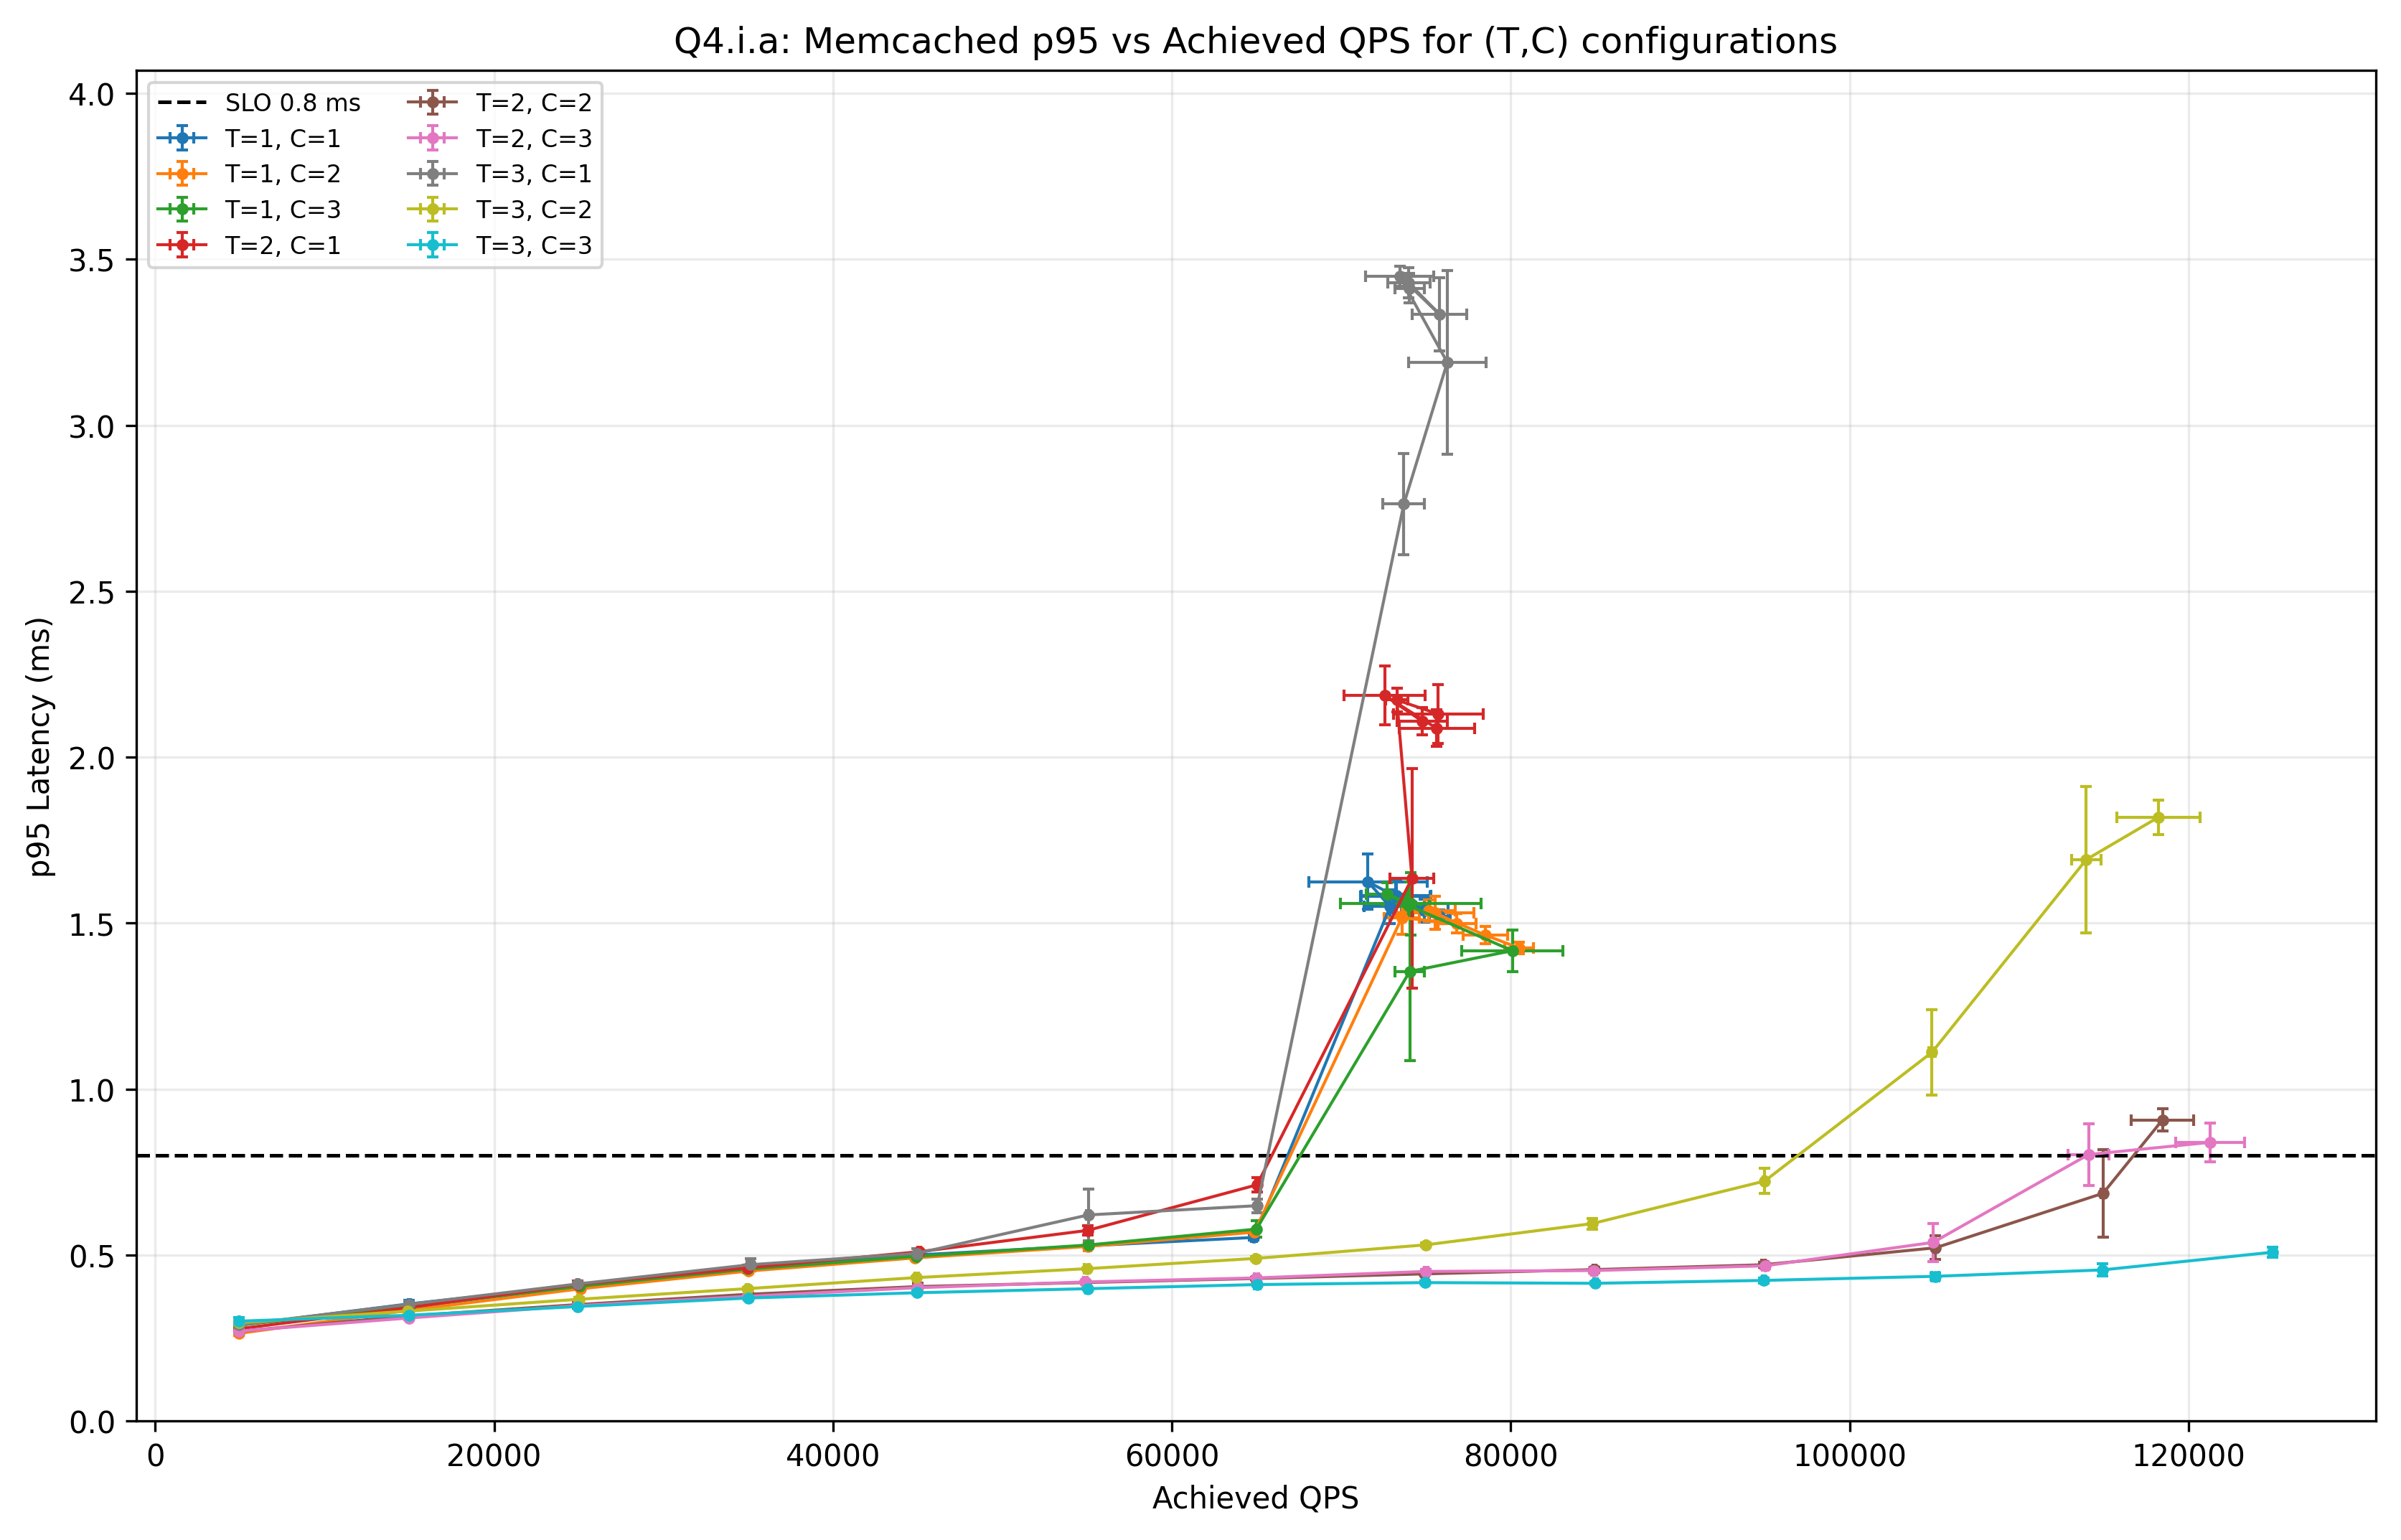
\includegraphics[width=0.75\linewidth]{figures/q4i_a.png}
        \caption{Memcached p95 latency vs. achieved QPS for different thread/core configurations.}
        \label{fig:1a}
    \end{figure}
        
    What do you conclude from the results in your plot? Summarize in 2-3 brief sentences how memcached performance varies with the number of threads and cores and how this relates to the target QPS.
    
    \textbf{Summary:} % Place your solution here.
    \\
    Figure \ref{fig:1a} shows that memcached performance depends on both the number of software threads and the number of CPU cores assigned to the process. Configurations with only one core become unstable beyond roughly 65k–75k QPS and violate the 0.8 ms p95 SLO. Increasing the number of cores without increasing the number of memcached threads provides little benefit, as shown by the similar behavior of T=1 with C=1, C=2, and C=3. Conversely, increasing the number of threads without providing enough cores leads to oversubscription and worsens tail latency, as observed for T=2,C=1 and T=3,C=1. The best configuration is T=3,C=3, which remains below the SLO even at the highest tested load. Therefore, our controller should reserve fewer cores for memcached at low load to maximize batch progress, but switch to T=2,C=2 or T=2,C=3 at medium/high load and to T=3,C=3 during high-load periods or when p95 approaches the SLO.
    
    b) [2 points] To support the highest load in the trace (around 125K QPS) without violating the 0.8ms latency SLO, how many memcached threads ($T$) and CPU cores ($C$) will you need?
    
    \textbf{Answer:} To support the highest load in the trace, around 125K QPS, without violating the 0.8 ms p95 latency SLO, we need $T=3$ memcached threads and $C=3$ CPU cores. This configuration is the only one that remains below the SLO at the highest tested loads.
    \\
    
    c) [1 point] Assume you can change the number of cores allocated to memcached dynamically as the QPS varies from 5K to 125K, but the number of threads is fixed when you launch the memcached job. How many memcached threads ($T$) do you propose to use to guarantee the 0.8ms 95th percentile latency SLO while the load varies between 5K to 125K QPS?
    
    \textbf{Answer:} We propose to use $T=3$ memcached threads. Since the number of threads is fixed at launch time, it must be chosen to handle the highest possible load. With $T=3$, the controller can dynamically vary the number of allocated cores between $C=1$, $C=2$, and $C=3$ as the QPS changes, while still being able to meet the 0.8 ms p95 latency SLO at high load.
    \\
    
    d) [8 points] Run memcached with the number of threads $T$ that you proposed in (c) and measure performance with $C=1$, $C=2$ and $C=3$. Use the aforementioned \texttt{mcperf} command to sweep QPS from 5K to 125K.

    Measure the CPU utilization on the memcached server at each load time step. Plot the performance of memcached using 1-core ($C=1$), 2 cores ($C=2$) and 3 ($C=3$) in \textbf{three separate graphs}, for $C=1$, $C=2$ and $C=3$, respectively. In each graph, plot achieved QPS on the x-axis, ranging from 0 to 125K. In each graph, use two y-axes. Plot the 95th percentile latency on the left y-axis. Draw a dotted horizontal line at the 0.8ms latency SLO. Plot the CPU utilization (ranging from 0\% to 100\% for $C=1$, 200\% for $C=2$ and 300\% for $C=3$) on the right y-axis. For simplicity, we do not require error bars for these plots. 
    
    \textbf{Plots:} % Place your plots here.
    \\
    \begin{figure}[H]
    \centering
    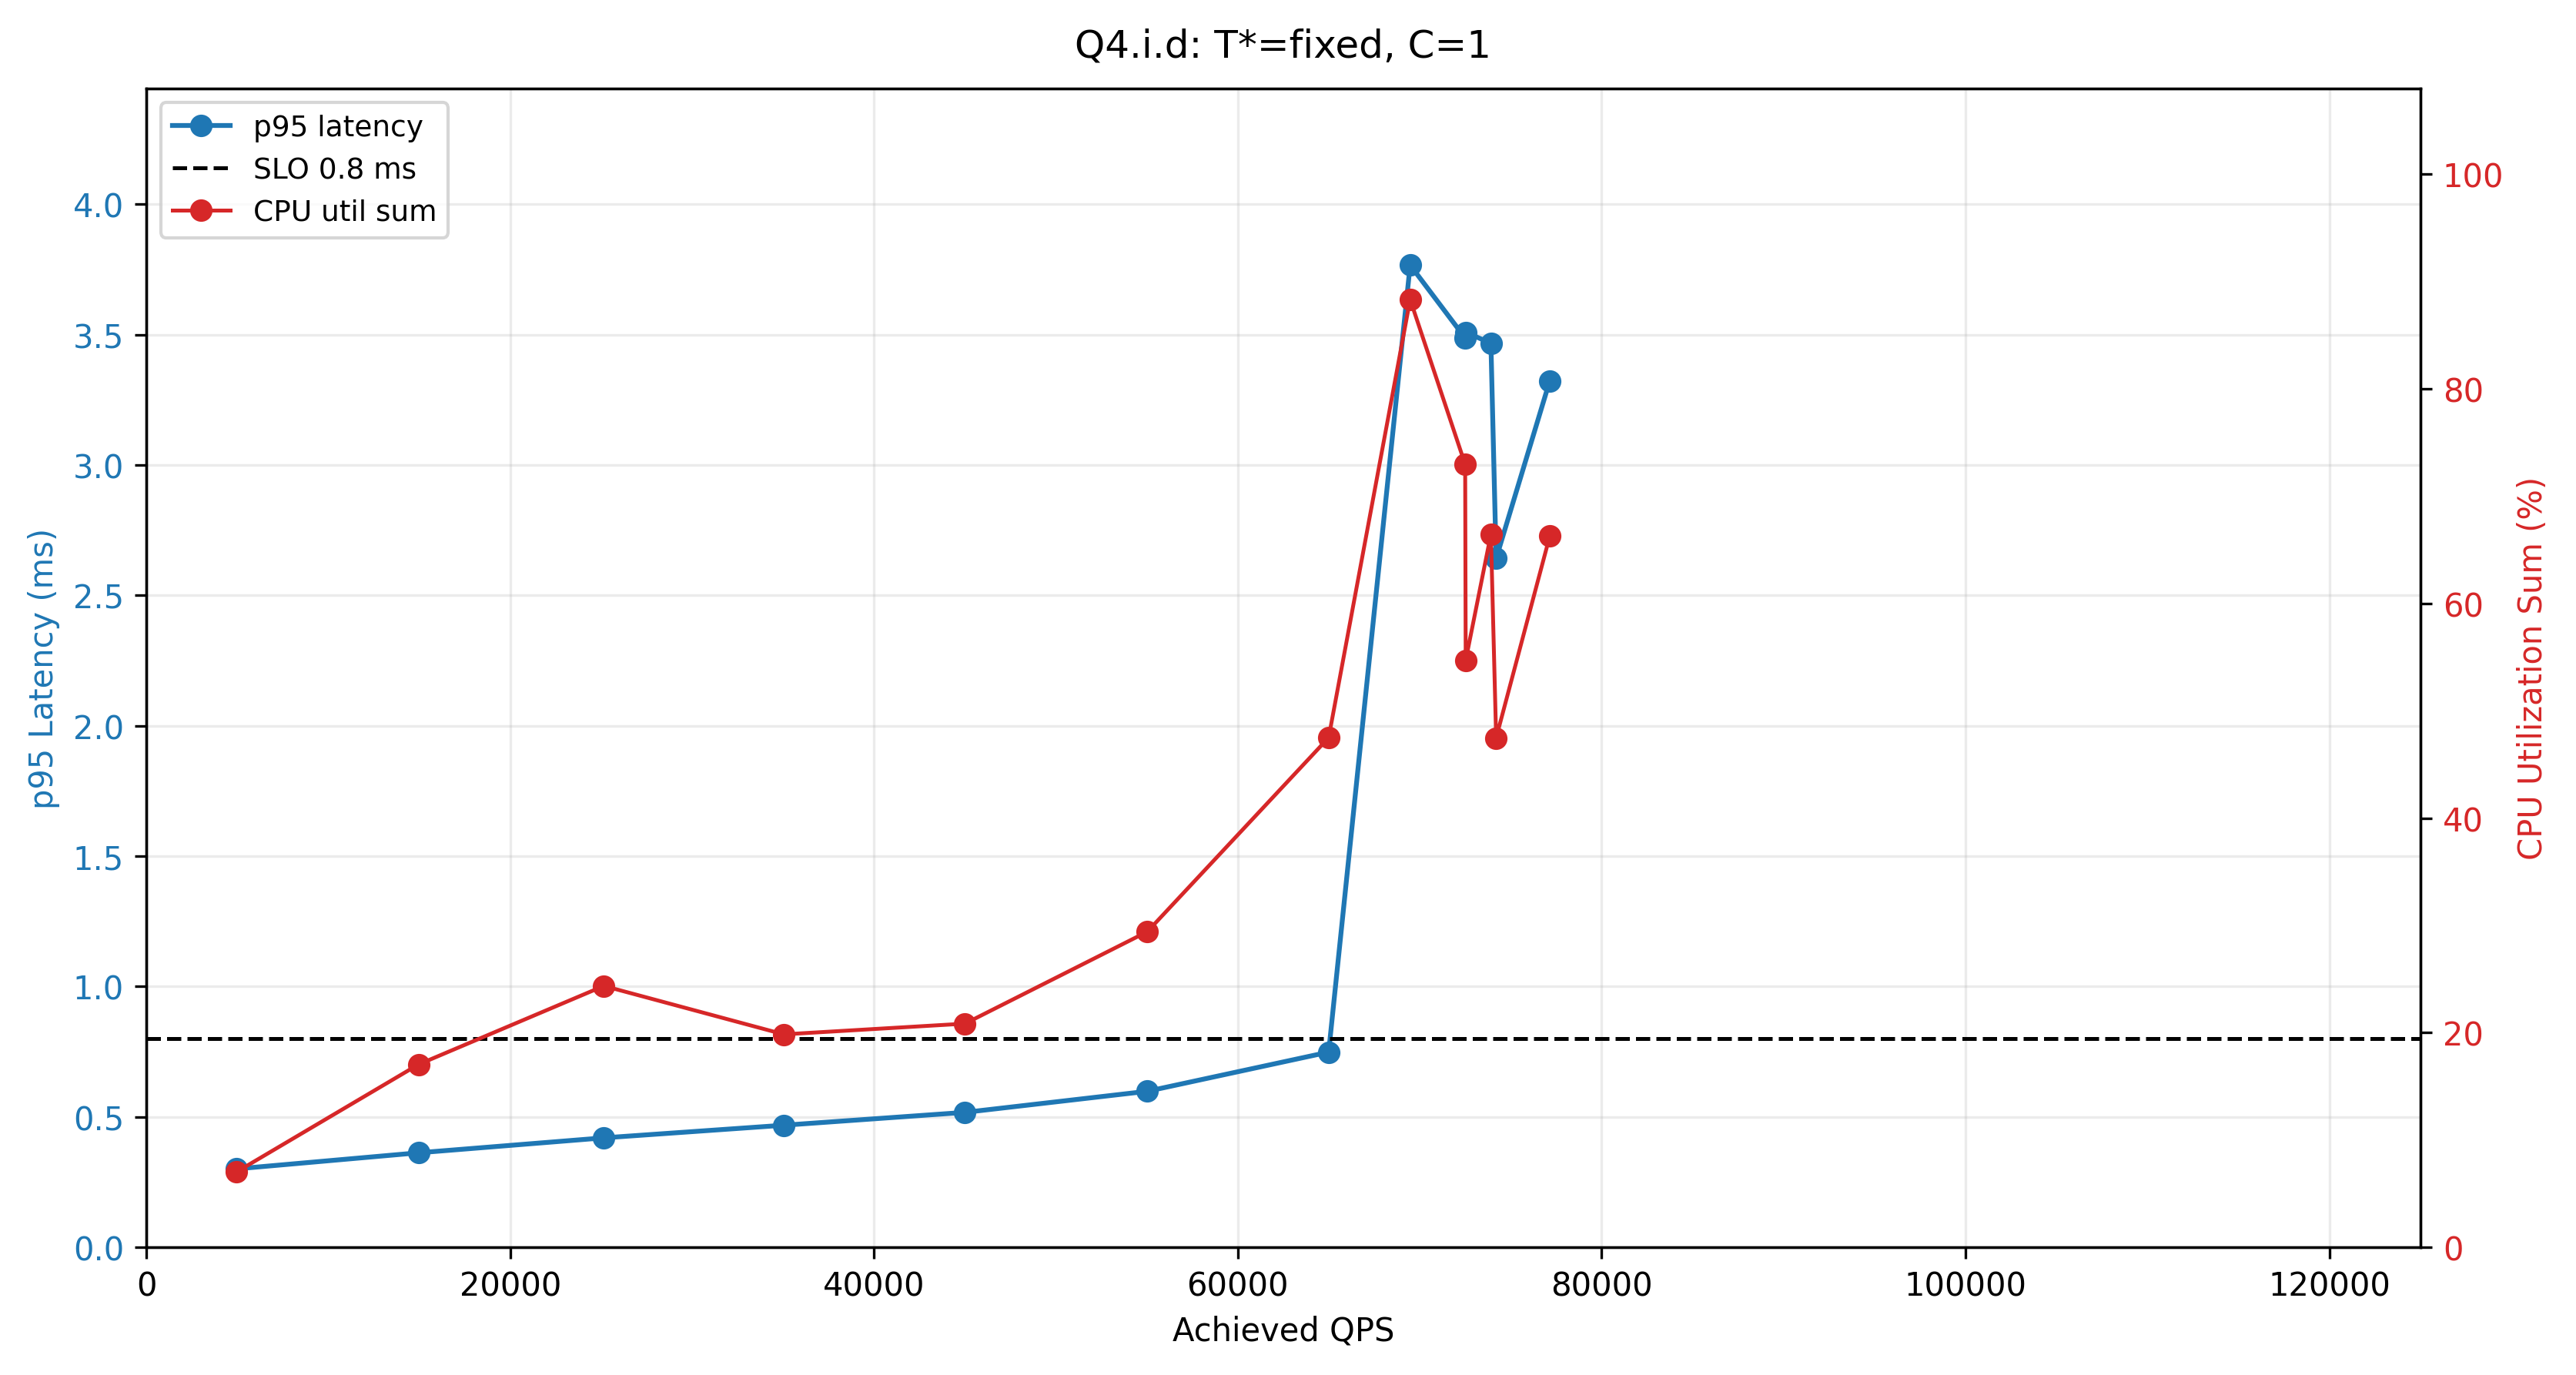
\includegraphics[width=0.65\linewidth]{figures/q4i_d_C1.png}
    \caption{Memcached p95 latency and CPU utilization versus achieved QPS with fixed $T=3$ and $C=1$.}
\end{figure}

\begin{figure}[H]
    \centering
    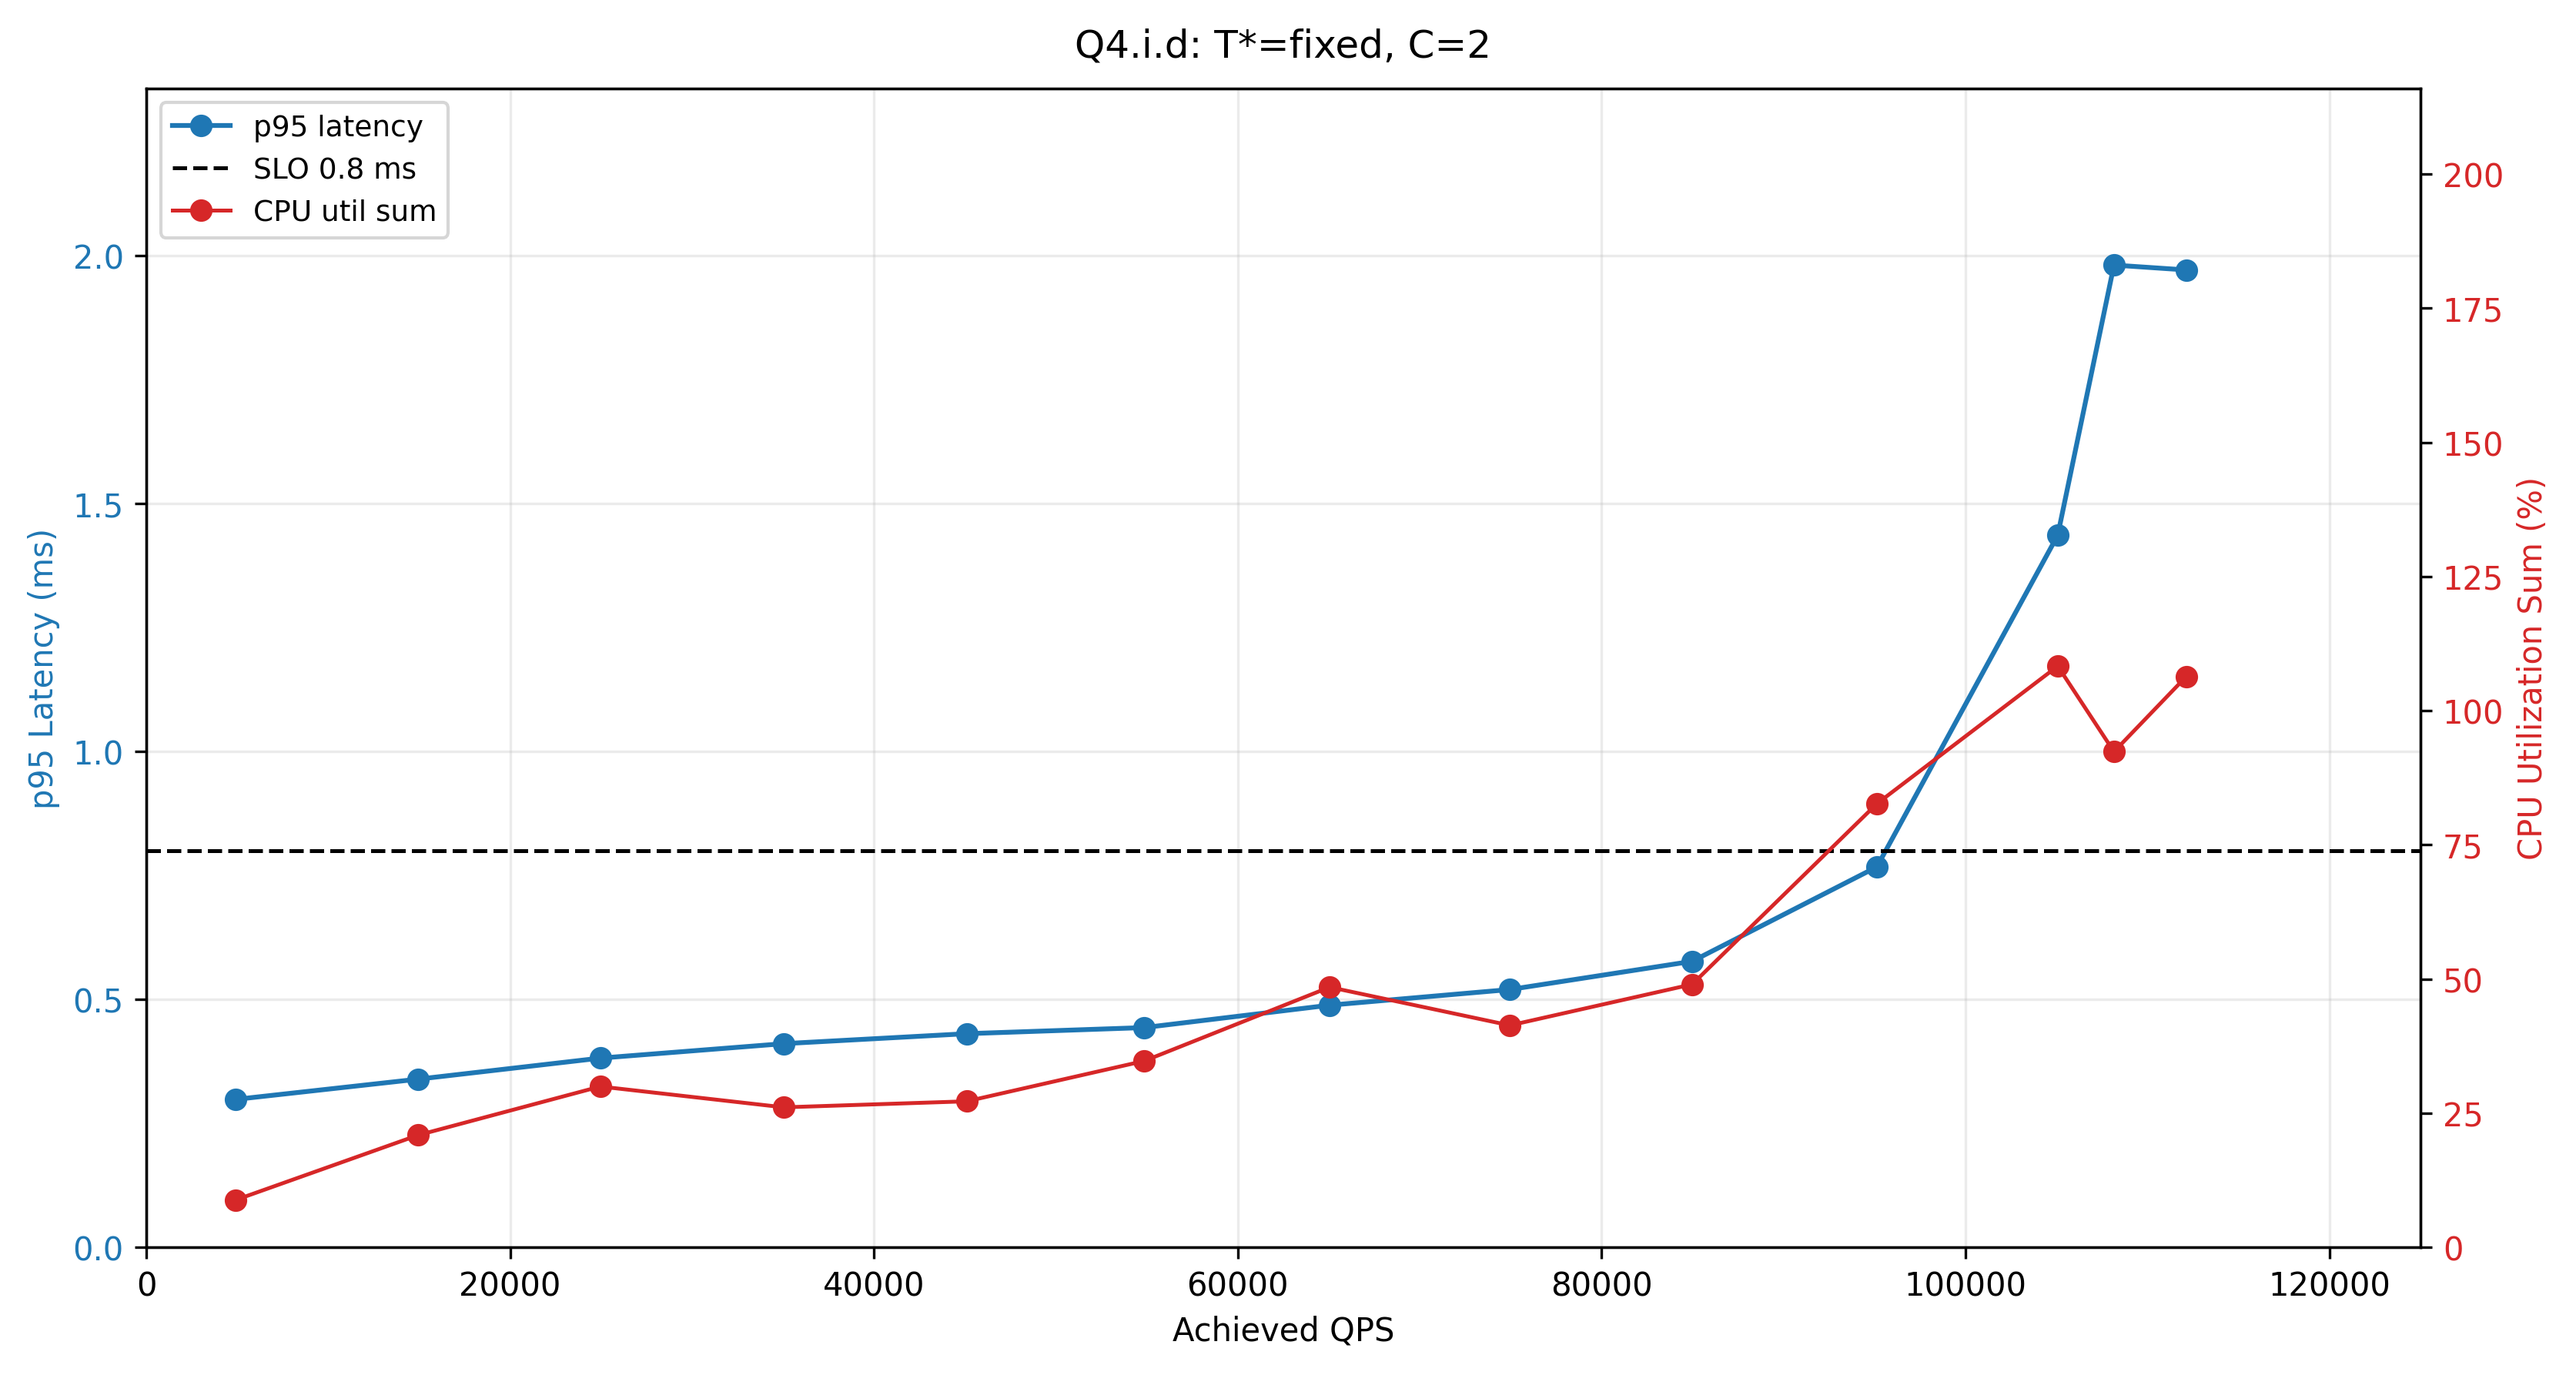
\includegraphics[width=0.65\linewidth]{figures/q4i_d_C2.png}
    \caption{Memcached p95 latency and CPU utilization versus achieved QPS with fixed $T=3$ and $C=2$.}
\end{figure}

\begin{figure}[H]
    \centering
    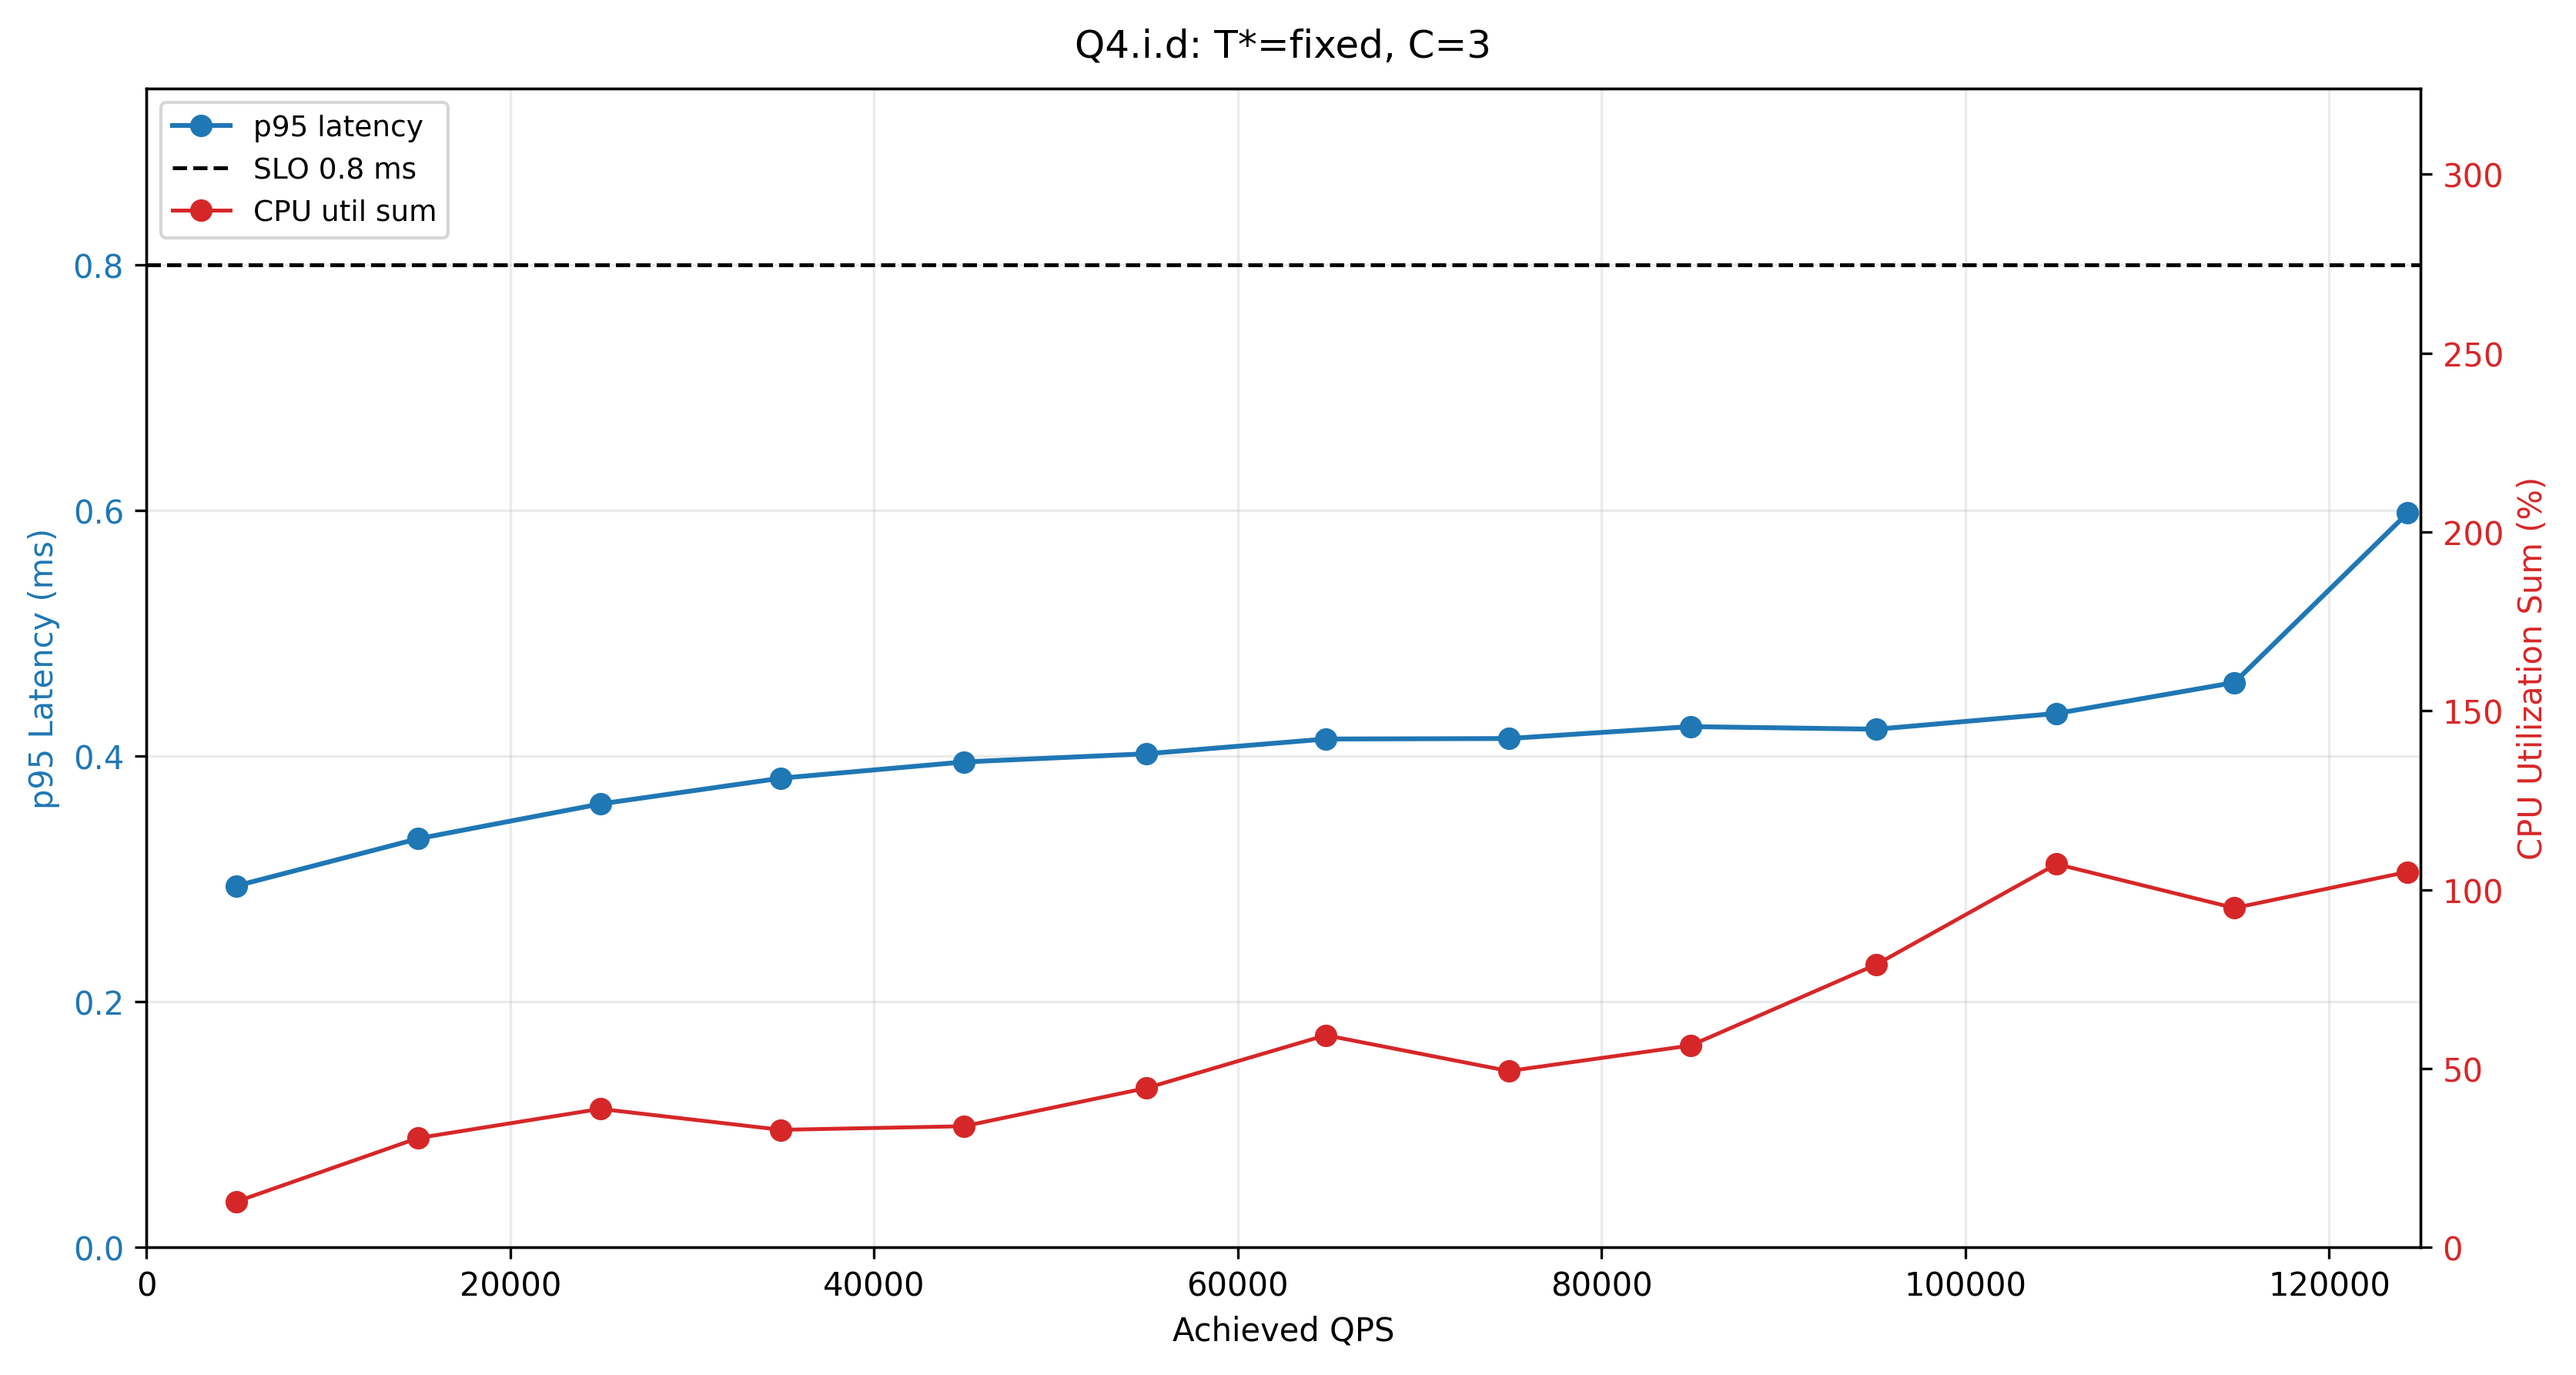
\includegraphics[width=0.65\linewidth]{figures/q4i_d_C3.png}
    \caption{Memcached p95 latency and CPU utilization versus achieved QPS with fixed $T=3$ and $C=3$.}
\end{figure}

With $T=3$ fixed, the results show that increasing the number of cores allocated to memcached significantly improves its ability to sustain higher QPS while respecting the 0.8 ms p95 latency SLO. With $C=1$, memcached quickly saturates and violates the SLO once the achieved QPS reaches roughly 70K. With $C=2$, the SLO is respected for a larger range, but the p95 latency exceeds 0.8 ms at high load. With $C=3$, memcached remains below the SLO across the full tested range up to approximately 125K QPS.



    
    \item \textbf{[17 points]} You are now given a dynamic load trace for memcached, which varies QPS randomly between 5K and 110K in 15 second time intervals. Use the following command to run this trace: 
        \begin{Verbatim}[fontsize=\small]
$ ./mcperf -s INTERNAL_MEMCACHED_IP --loadonly 
$ ./mcperf -s INTERNAL_MEMCACHED_IP -a INTERNAL_AGENT_IP \ 
           --noload -T 8 -C 8 -D 4 -Q 1000 -c 8 -t 1800 \ 
           --qps_interval 15 --qps_min 5000 --qps_max 110000
\end{Verbatim}
    
    Note that you can also specify a random seed in this command using the \texttt{--qps\_seed} flag. 

    For this and the next questions, feel free to reduce the mcperf measurement duration (\texttt{-t} parameter, now fixed to 30 minutes) as long as you have at the end at least 1 minute of memcached running alone.
    \\
    
    Design and implement a controller to schedule memcached and the benchmarks (batch jobs) on the 4-core VM. The goal of your scheduling policy is to successfully complete all batch jobs as soon as possible without violating the 0.8ms 95th percentile latency for memcached. \textbf{Your controller should not assume prior knowledge of the dynamic load trace. You should design your policy to work well regardless of the random seed.} The batch jobs need to use the native dataset, i.e., provide the option \texttt{-i native} when running them. Also make sure to check that all the batch jobs complete successfully and do not crash. Note that batch jobs may fail if given insufficient resources. \\
    
    Describe how you designed and implemented your scheduling policy. Include the source code of your controller in the zip file you submit. 

    \begin{itemize}
        \item Brief overview of the scheduling policy (max 10 lines):
        
    \textbf{Answer:}
    Our controller samples memcached CPU usage every 1 s and dynamically changes the number of cores assigned to memcached between 1 and 3. Memcached is pinned to the low-numbered cores, while Docker batch jobs are restricted to the remaining cores using cpuset updates. The policy prioritizes SLO protection: memcached cores are increased immediately under high per-core CPU load, while cores are released only after sustained low load. To reduce makespan, the final policy uses an opportunistic overlap mode: when memcached needs only one core, the two long critical-path jobs, \colored{streamcluster} and \colored{freqmine}, are allowed to run concurrently with a companion job. When memcached needs two or three cores, the policy falls back to a more conservative schedule. The controller does not use future QPS values; it reacts only to runtime CPU signals.
     
    \item How do you decide how many cores to dynamically assign to memcached? Why?
    
    \textbf{Answer:}
Memcached uses a fixed thread count of $T^*=3$ and dynamically receives $C_{mem}\in\{1,2,3\}$. The controller starts with $C_{mem}=2$. Every second it computes memcached CPU utilization per assigned core. If utilization exceeds $85\%$ per core, $C_{mem}$ is increased immediately, up to 3 cores, to protect the 0.8 ms p95 latency SLO. If utilization stays below $55\%$ per core for 20 seconds, $C_{mem}$ is reduced by one, down to 1 core, to give more capacity back to batch jobs. This hysteresis avoids oscillations while still reacting quickly to high QPS.

    \item How do you decide how many cores to assign each batch job? Why?

     \textbf{Answer:}
All batch jobs run only on cores not currently used by memcached. If $C_{mem}=1$, batch jobs can use cores $[1,2,3]$; if $C_{mem}=2$, they use $[2,3]$; if $C_{mem}=3$, only core $[3]$ is available. The final policy uses these cores opportunistically: at low memcached load ($C_{mem}=1$), it overlaps the two long jobs to shorten the critical path; at medium/high memcached load, it schedules more conservatively to protect the SLO.


\begin{itemize}
    \item \colored{barnes}: short/risky companion job; usually 1 core when collocated, more only when long jobs are done.
    \item \colored{blackscholes}: short and relatively safe; 1 core when collocated, up to 2 cores due to weak scaling beyond that.
    \item \colored{canneal}: memory-bandwidth style job; used as a companion at low/medium memcached load, but not launched while $C_{mem}=3$.
    \item \colored{freqmine}: long critical-path job; overlapped with \colored{streamcluster} when memcached has enough headroom, but paused first under high memcached pressure.
    \item \colored{radix}: safest short job; can run even when memcached uses 3 cores.
    \item \colored{streamcluster}: long critical-path job; started early and overlapped with \colored{freqmine} during low-load periods.
    \item \colored{vips}: short but CPU/L1i-risky; scheduled after safer short jobs and may be paused under high load.
\end{itemize}

    \item How many threads do you use for each of the batch job? Why?
Threads are usually set equal to the number of assigned cores, capped by the per-job maximum. In the opportunistic low-load mode, \colored{streamcluster} and \colored{freqmine} use at least 2 software threads even when each receives one core; this kept both long jobs making progress and reduced makespan in our experiments.

\begin{itemize}
    \item \colored{barnes}: $\min(\text{assigned cores},4)$
    \item \colored{blackscholes}: $\min(\text{assigned cores},2)$
    \item \colored{canneal}: $\min(\text{assigned cores},2)$
    \item \colored{freqmine}: $\min(\max(\text{assigned cores},2),4)$ in opportunistic mode
    \item \colored{radix}: $\min(\text{assigned cores},4)$
    \item \colored{streamcluster}: $\min(\max(\text{assigned cores},2),4)$ in opportunistic mode
    \item \colored{vips}: $\min(\text{assigned cores},4)$
\end{itemize}

      
    \item Which jobs run concurrently / are collocated and on which cores? Why?

    \textbf{Answer:}
Memcached always uses the low-numbered cores $[0..C_{mem}-1]$. Batch jobs use only the remaining high-numbered cores. When $C_{mem}=1$, the controller can use cores 1--3 and may collocate \colored{streamcluster}, \colored{freqmine}, and one companion job. When $C_{mem}=2$, it usually runs one long job plus one companion job. When $C_{mem}=3$, only one safe/useful batch job runs on the remaining core, preferring \colored{radix} or \colored{blackscholes}. This keeps risky interference away from memcached during high load while exploiting low-load periods to shorten the batch critical path.

    \item In which order did you run the batch jobs? Why?

\textbf{Order} (to be sorted):
\colored{streamcluster}, \colored{freqmine}, \colored{canneal},
\colored{radix}, \colored{blackscholes}, \colored{barnes}, \colored{vips}





    \textbf{Why:}
    The policy prioritizes \colored{streamcluster} and \colored{freqmine} because they are the longest critical-path jobs, so delaying them increases makespan. \colored{canneal} is started as a companion when enough memcached headroom exists, but it is blocked when memcached needs 3 cores. Among short jobs, \colored{radix} and \colored{blackscholes} are scheduled early because they are safer for memcached, while \colored{barnes} and \colored{vips} are more CPU/L1i-risky and are therefore scheduled later or paused under pressure.

\item How does your policy differ from the policy in Part 3? Why?

\textbf{Answer:} Part 3 used a static schedule and fixed resource assignment for a fixed-load scenario. Part 4 uses a dynamic QPS trace on one 4-core VM, so a static assignment would either waste cores at low QPS or violate the memcached SLO at high QPS. The Part 4 controller therefore continuously adjusts memcached cores, updates Docker cpusets for batch jobs, and uses pause/unpause as a recovery mechanism. In addition, unlike Part 3, it opportunistically overlaps the long batch jobs only when memcached has enough headroom, and falls back to a conservative schedule when memcached load increases.


\item How did you implement your policy? e.g., docker cpu-set updates, taskset updates for memcached, pausing/unpausing containers, etc.

\textbf{Answer:} The controller runs on the memcache-server VM. Memcached is controlled with \texttt{taskset} to update its CPU affinity. Batch jobs are launched as Docker containers with the native input dataset and fixed cpusets. While running, the controller uses Docker cpuset updates to move containers to the currently available batch cores. If memcached per-core CPU exceeds the recovery threshold, the controller pauses the riskiest running container; it unpauses paused containers once memcached utilization falls below the recovery threshold and the job is still part of the desired schedule. All start, end, pause, unpause, and core-update events are logged.

\item Describe the design choices, ideas and trade-offs you took into account while creating your scheduler (\underline{if not already mentioned above}). Describe how your policy (and its performance) compares to another policy that you experimented with (in particular to the second-best policy that you designed).

\textbf{Answer:} The main trade-off is makespan versus memcached SLO protection. The original conservative policy completed Q4.iii in $1208.52\pm33.00$ s with no SLO violations, but it left too much critical-path work serialized. We therefore tested a more aggressive policy that always overlapped the two long jobs; it reduced makespan in some runs but produced SLO violations above the 3\% target. The final opportunistic-overlap policy keeps this overlap only when memcached has been reduced to one core, and falls back to the conservative schedule when memcached needs more protection. With this design, Q4.iii improved to $968.19\pm23.20$ s while keeping the SLO violation ratio at $0.0\%$ in all three runs.
\end{itemize}

\item \textbf{[23 points]} Run the following \texttt{mcperf} memcached dynamic load trace: 
    
\begin{Verbatim}[fontsize=\small]
$ ./mcperf -s INTERNAL_MEMCACHED_IP --loadonly 
$ ./mcperf -s INTERNAL_MEMCACHED_IP -a INTERNAL_AGENT_IP \ 
           --noload -T 8 -C 8 -D 4 -Q 1000 -c 8 -t 1800 \ 
           --qps_interval 15 --qps_min 5000 --qps_max 110000 \ 
           --qps_seed 2345
\end{Verbatim}
    
    
    Measure memcached and batch job performance when using your scheduling policy to launch workloads and dynamically adjust container resource allocations. Run this workflow 3 separate times. For each run, measure the execution time of each batch job, as well as the latency outputs of memcached. For each batch application, compute the mean and standard deviation of the execution time \footnote{Here, you should only consider the runtime, excluding time spans during which the container is paused.} across three runs. Compute the mean and standard deviation of the total time to complete all jobs - the makespan of all jobs. Fill in the table below.  Also, compute the SLO violation ratio for memcached for each of the three runs; the number of data points with 95th percentile latency $>$ 0.8ms, as a fraction of the total number of datapoints. The SLO violation ratio should be calculated during the time from when the first batch-job-container starts running to when the last batch-job-container stops running. \\
    
    \begin{table}[ht]
        \centering
        \begin{tabular}{ |c|c|c|c|c|} 
            \hline
            job name & mean time [s] & std [s] \\ \hline \hline
            \coloredcell{barnes}          & 190.75 & 0.53 \\ \hline
            \coloredcell{blackscholes}    & 118.64 & 0.48 \\ \hline
            \coloredcell{canneal}         & 289.54 & 1.32 \\ \hline
            \coloredcell{freqmine}        & 419.88 & 23.70 \\ \hline
            \coloredcell{radix}           & 44.99  & 0.59 \\ \hline
            \coloredcell{streamcluster}   & 543.76 & 7.14 \\ \hline
            \coloredcell{vips}            & 94.21  & 0.37 \\ \hline
            total time                    & 968.19 & 23.20 \\ \hline
        \end{tabular}
    \end{table}

    \textbf{Answer:}
    We ran the dynamic mcperf trace with $qps\_interval=15$ and $qps\_seed=2345$ three times using our dynamic controller. All seven batch jobs completed successfully in every run. The reported job runtimes exclude time spent paused. The mean makespan over the three runs was $968.19$ s with a standard deviation of $23.20$ s. The memcached SLO violation ratio was $0.0\%$ in all three runs: run 1 = $0.0\%$, run 2 = $0.0\%$, run 3 = $0.0\%$. Therefore, the controller met the 0.8 ms p95 latency SLO while completing all batch jobs.

    Include three plots: one for each of the three runs with the following information: The x-axis should be the time from execution start to end. Use three subplots that share the same x-axis. The first should clearly indicate for each core what job it is running at all time (e.g. using colored boxes). Use the colors proposed in this template (you can find them in \texttt{main.text}). If you pause/unpause jobs as part of your scheduling policy this should also be clearly visible. The second subplot should include two y-axis where the left one shows the current QPS and the right one should include the achieved p95 latency. Finally, the third subplot should plot the cpu utilization of each core separately. The readability of your plot will be part of awarded points.
    %Include six plots -- two plots for each of the three runs -- with the following information. Label the plots as 1A, 1B, 2A, 2B, 3A, and 3B where the number indicates the run and the letter indicates the type of plot (A or B), which we describe below. In all plots, time will be on the x-axis and you should annotate the x-axis to indicate which benchmark (batch) application starts executing at which time. If you pause/unpause any workloads as part of your policy, you should also indicate the timestamps at which jobs are paused and unpaused. All the plots will have have two y-axes. The right y-axis will be QPS. For Plots A, the left y-axis will be the 95th percentile latency. For Plots B, the left y-axis will be the number of CPU cores that your controller allocates to memcached. For the plot, use the colors proposed in this template (you can find them in \texttt{main.tex}).
\newpage
   \textbf{Plots:} 
\begin{figure}[H]
    \centering
    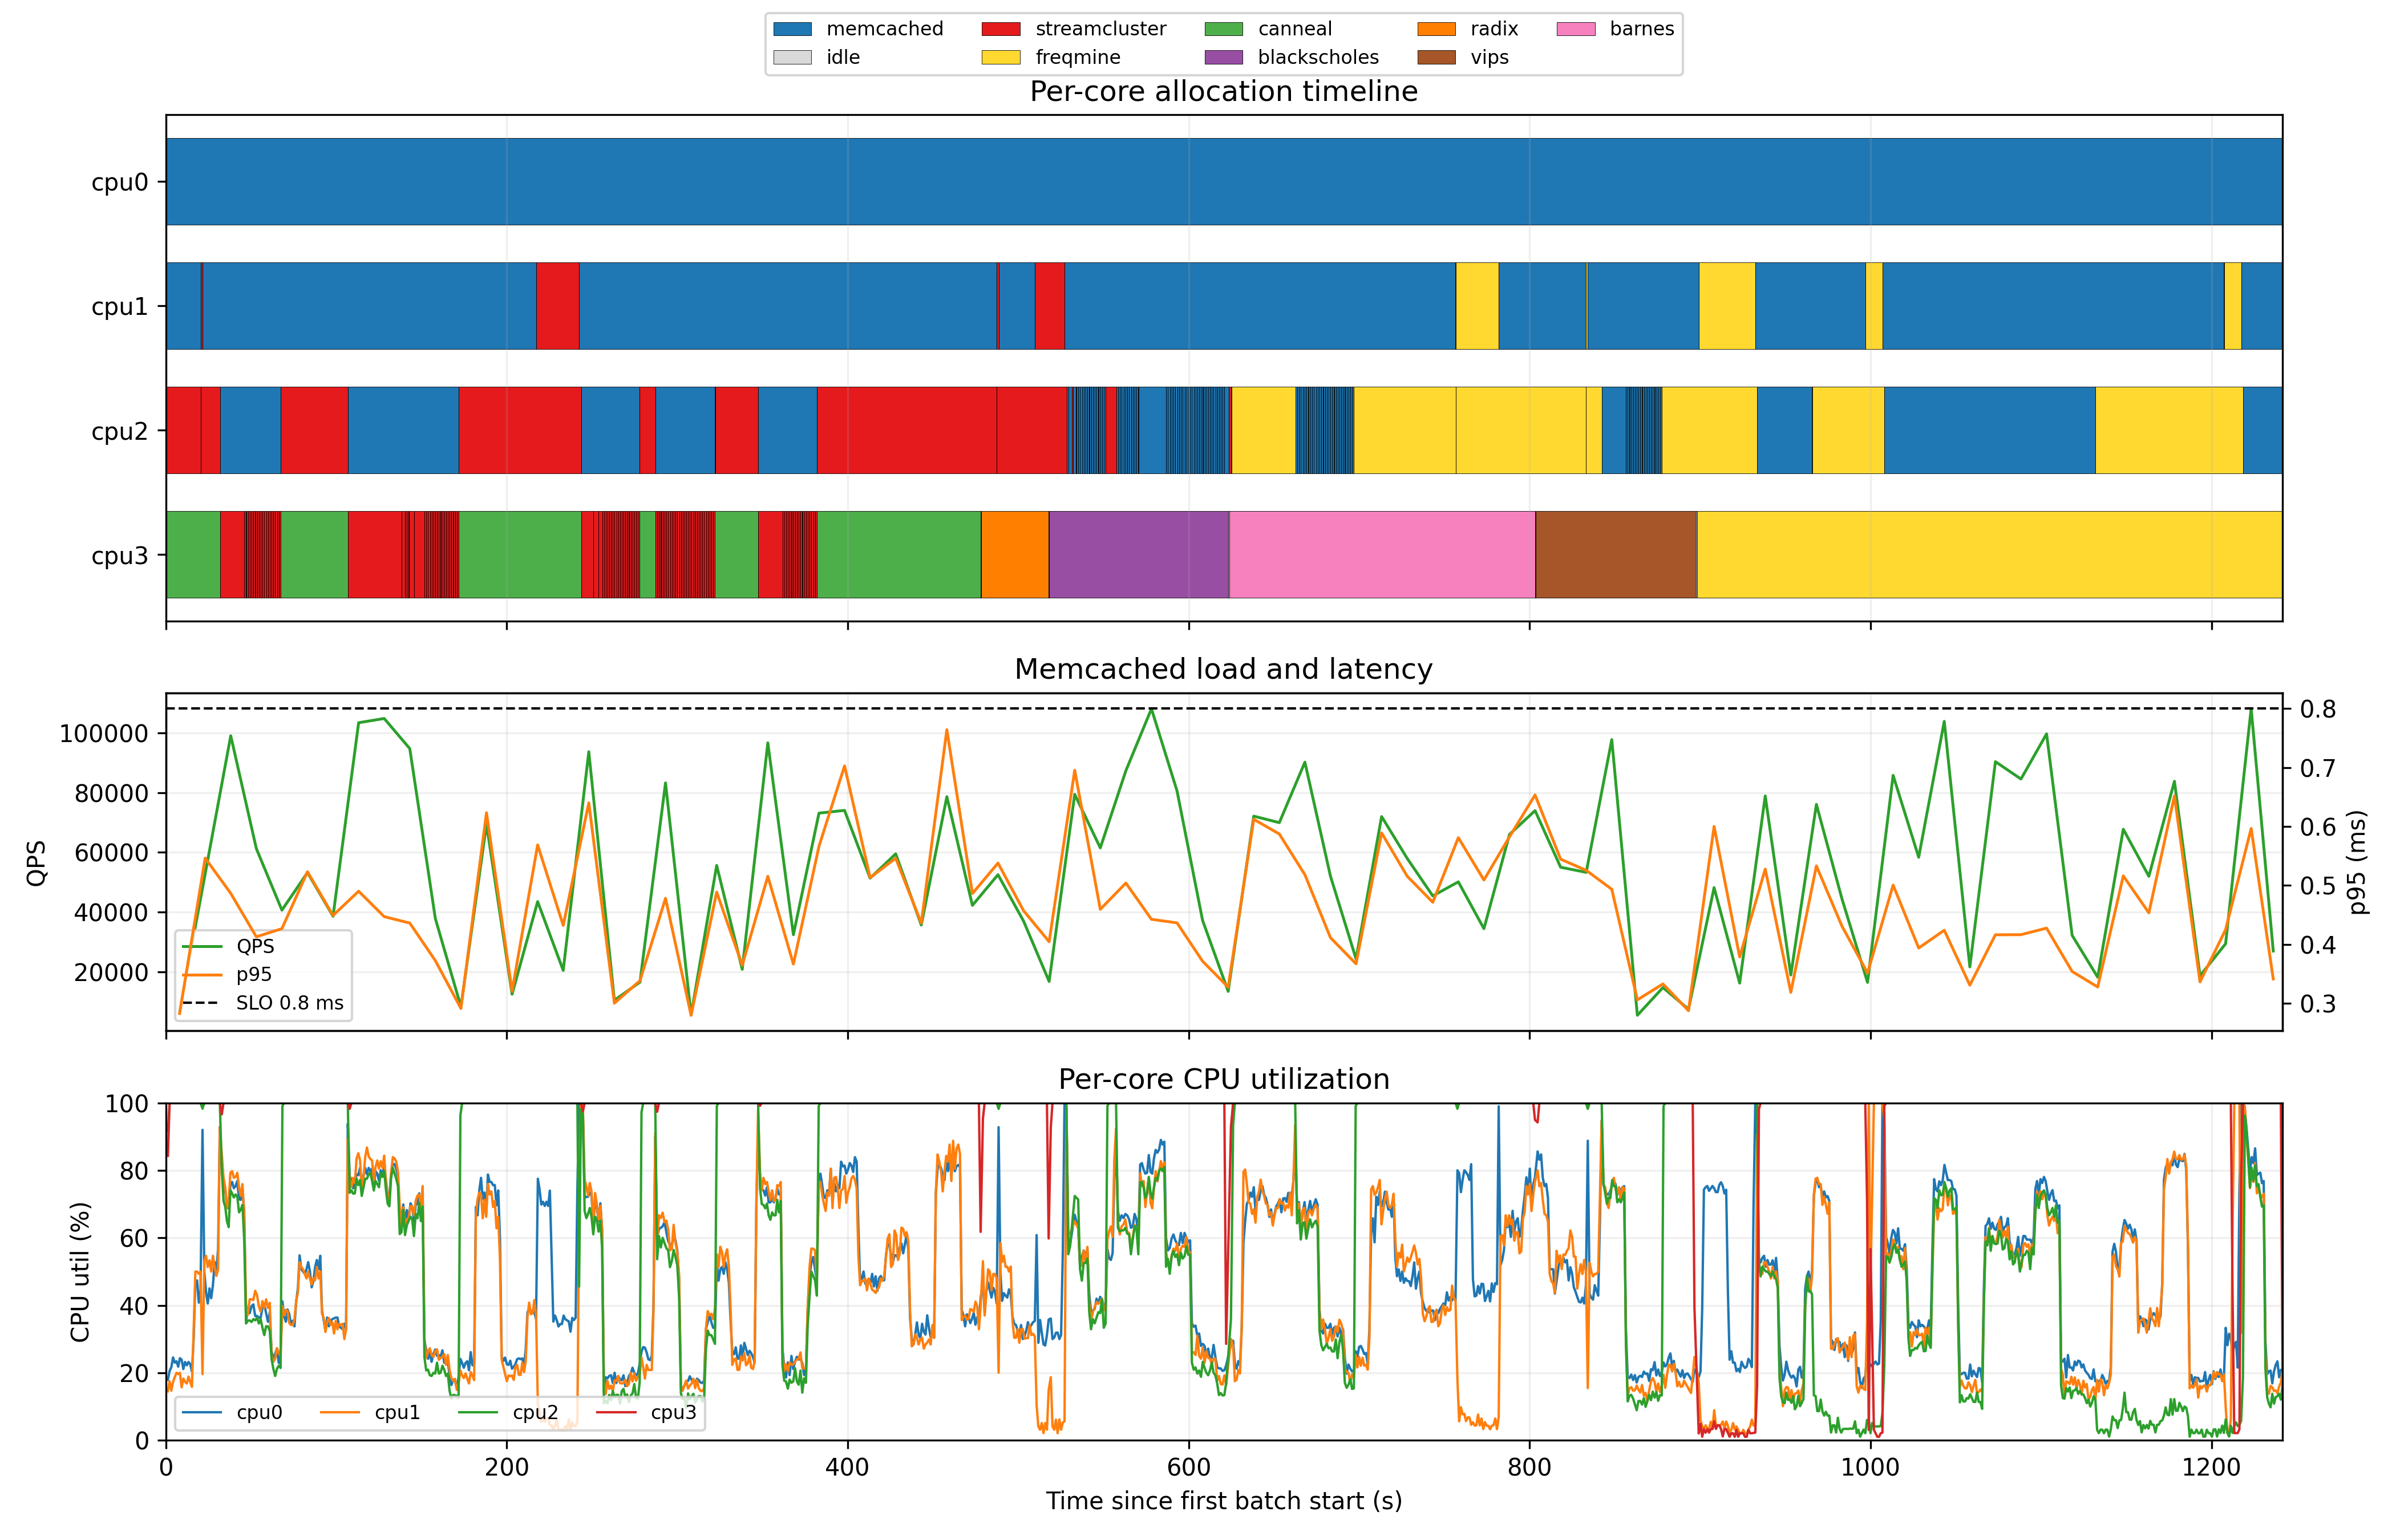
\includegraphics[width=0.75\linewidth]{figures/q4iii_run_1.png}
    \caption{Q4.iii run 1.}
\end{figure}

\begin{figure}[H]
    \centering
    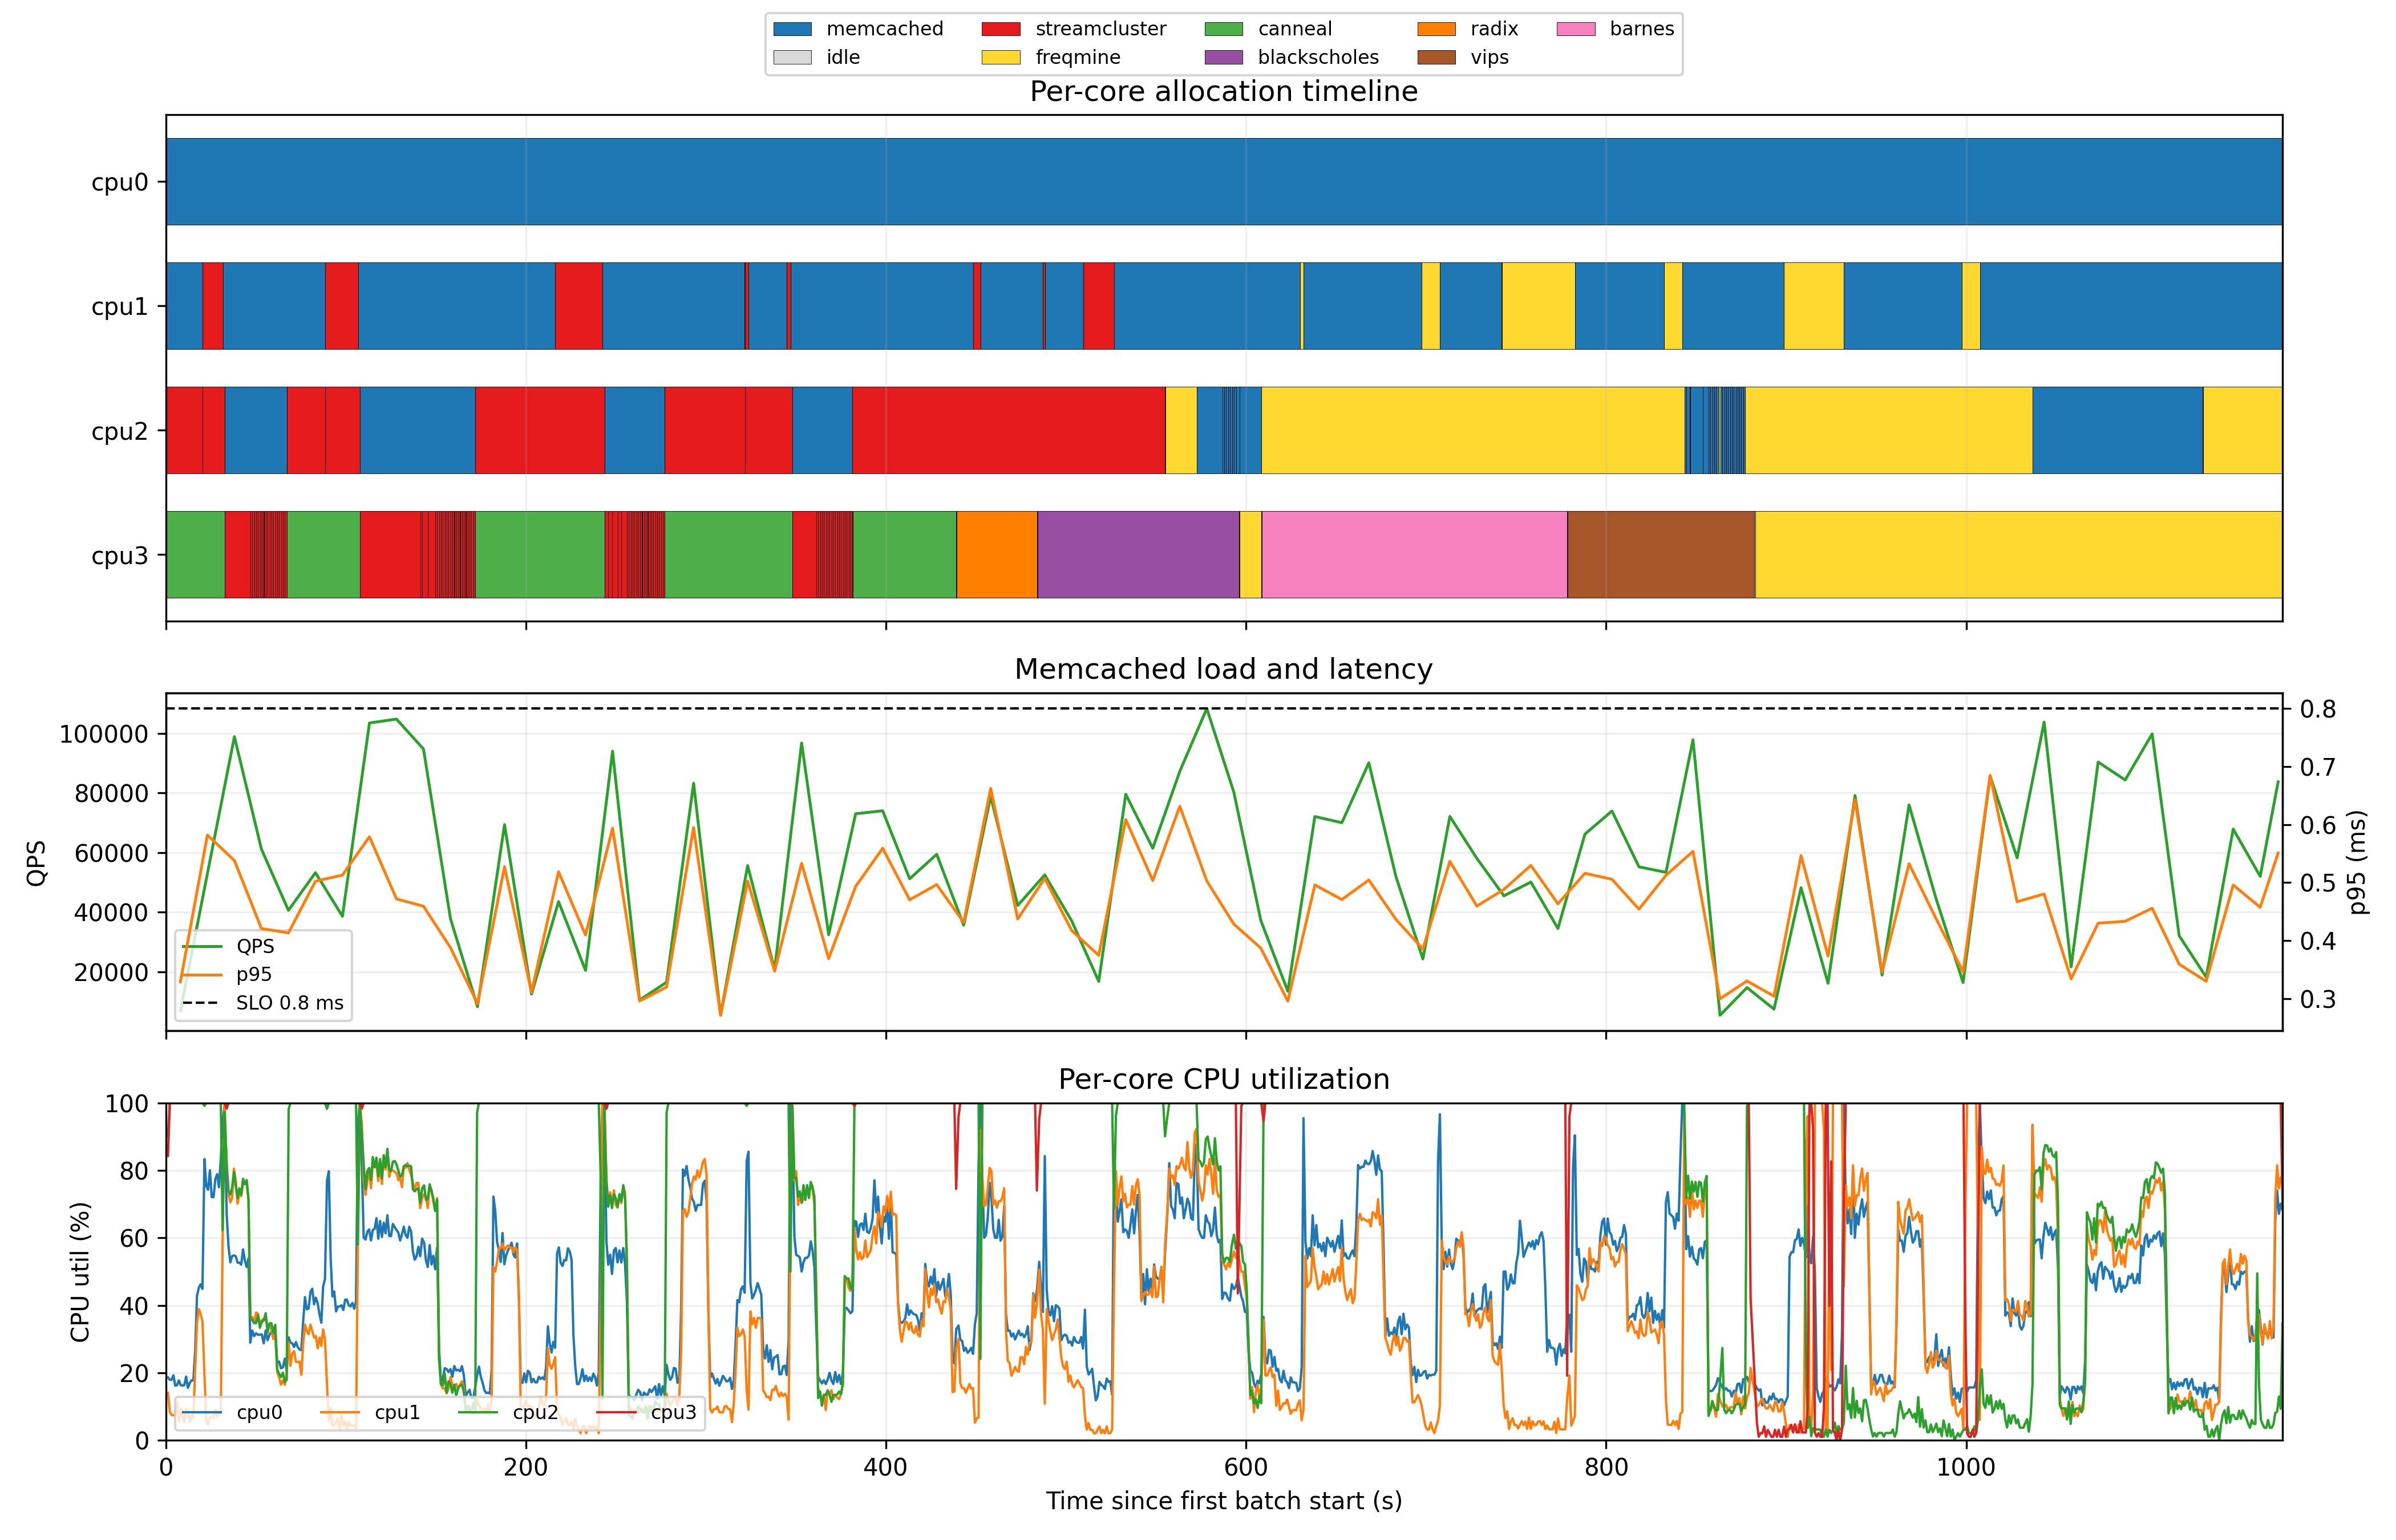
\includegraphics[width=0.75\linewidth]{figures/q4iii_run_2.png}
    \caption{Q4.iii run 2.}
\end{figure}

\begin{figure}[H]
    \centering
    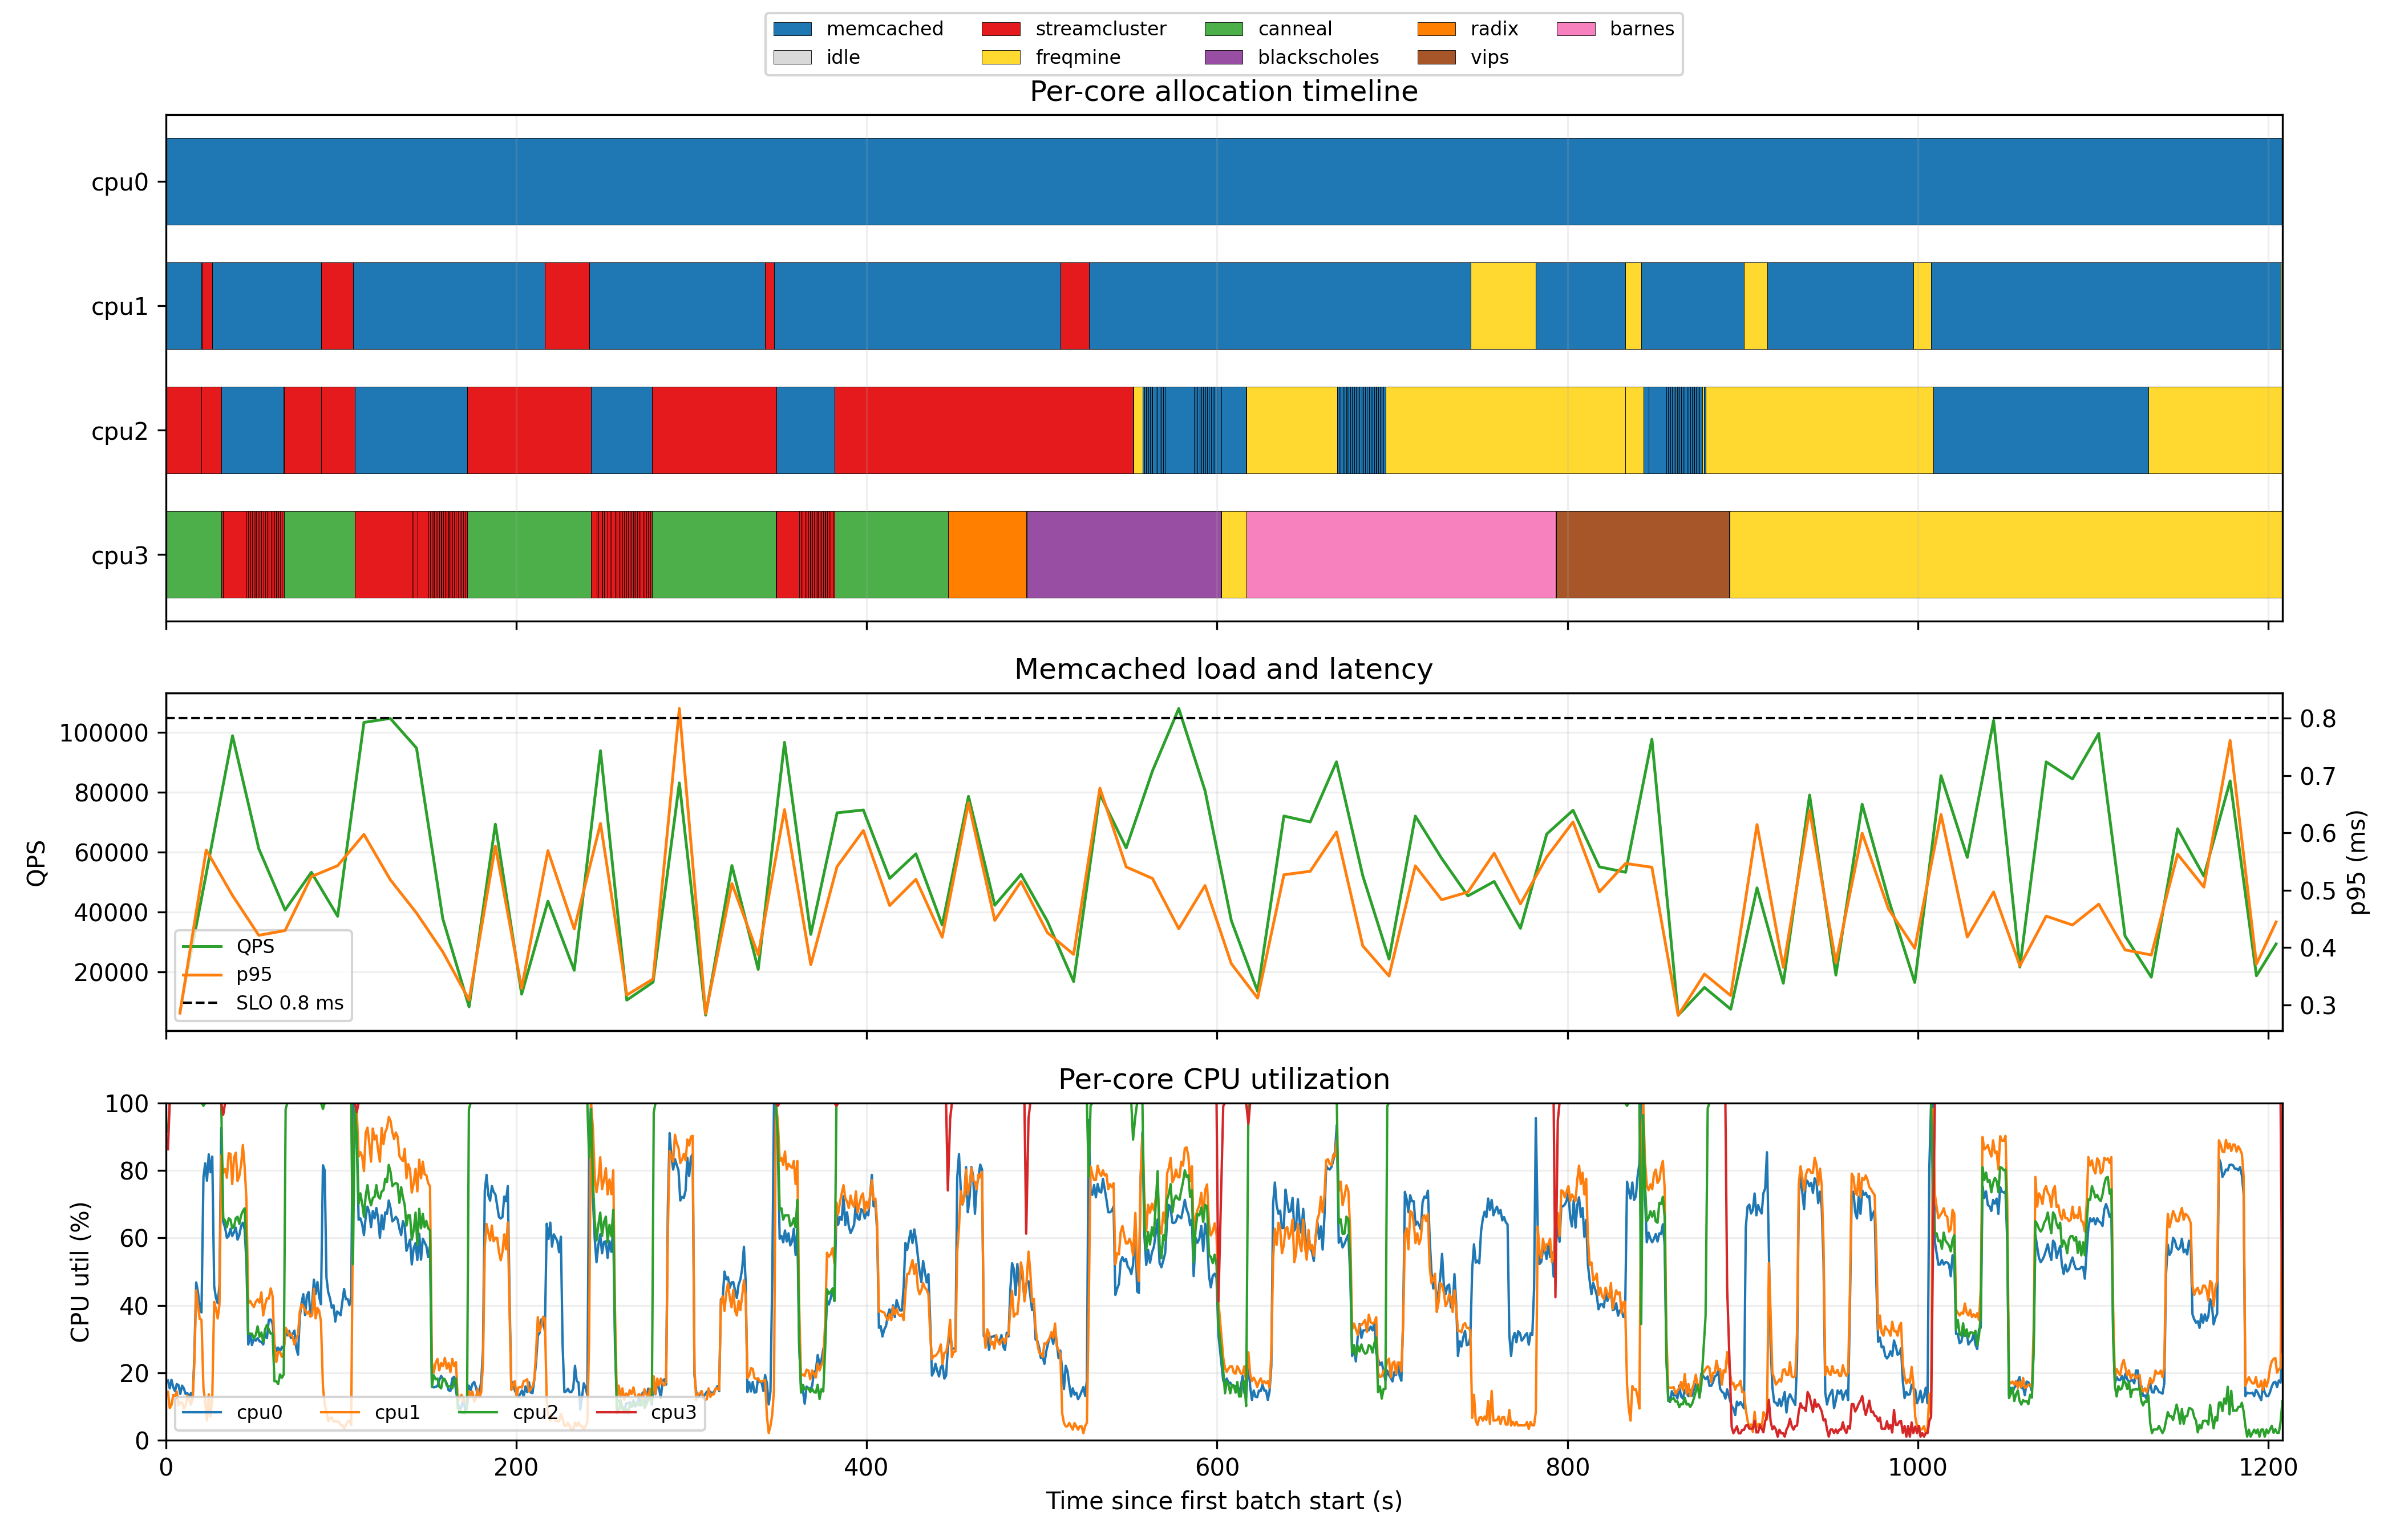
\includegraphics[width=0.75\linewidth]{figures/q4iii_run_3.png}
    \caption{Q4.iii run 3.}
\end{figure}


    \item \textbf{[16 points]} Repeat Part 4 Question 3 with a modified \texttt{mcperf} dynamic load trace with a 5 second time interval (\texttt{qps\_interval}) instead of 15 second time interval. Use the following command: 
    
\begin{Verbatim}[fontsize=\small]
$ ./mcperf -s INTERNAL_MEMCACHED_IP --loadonly 
$ ./mcperf -s INTERNAL_MEMCACHED_IP -a INTERNAL_AGENT_IP \ 
           --noload -T 8 -C 8 -D 4 -Q 1000 -c 8 -t 1800 \ 
           --qps_interval 5 --qps_min 5000 --qps_max 110000 \ 
           --qps_seed 2345
\end{Verbatim}
    
    You do not need to include the plots or table from Question 3 for the 5-second interval. Instead, summarize in 2-3 sentences how your policy performs with the smaller time interval (i.e., higher load variability) compared to the original load trace in Question 3. 

    \textbf{Summary:} 
    With $qps\_interval=5$, the load changes more frequently than in Question 3, so the controller has less time to react and keeps or returns CPU capacity to memcached more aggressively. This increases pressure on the scheduler compared with the 15 s trace, but the controller still keeps memcached below the required 3\% SLO violation threshold. In the 5 s sweep run, the SLO violation ratio was $0.76\%$, compared with $0.0\%$ average for the original 15 s trace.

    What is the SLO violation ratio for memcached (i.e., the number of datapoints with 95th percentile latency $>$ 0.8ms, as a fraction of the total number of datapoints) with the 5-second time interval trace? The SLO violation ratio should be calculated during the time from when the first batch-job-container starts running to when the last batch-job-container stops running.

    \textbf{Answer:} The SLO violation ratio for the 5-second interval trace was $0.00756$, i.e. $0.76\%$.

    What is the smallest \texttt{qps\_interval} you can use in the load trace that allows your controller to respond fast enough to keep the memcached SLO violation ratio under 3\%? 
    
    \textbf{Answer:} The smallest tested \texttt{qps\_interval} that kept the memcached SLO violation ratio below $3\%$ was $1$ second.

    What is the reasoning behind this specific value? Explain which features of your controller affect the smallest \texttt{qps\_interval} interval you proposed.

    \textbf{Answer:}We tested intervals $15,10,7,5,3,2,1$ seconds. The controller still stayed below the $3\%$ SLO violation threshold at $1$ second: the sweep run had $0.95\%$ violations. This works because the controller samples CPU utilization every second, immediately increases memcached's CPU allocation when pressure is high, and pauses/unpauses batch jobs when memcached needs protection. The main limiting factor is this 1-second control loop and the overhead of changing Docker cpusets and memcached taskset assignments; below 1 second the load could change faster than the controller can reliably observe and react.

    % Use this \texttt{qps\_interval} in the command above and collect results for three runs and fill out the table below. %Include the same types of plots (1A, 1B, 2A, 2B, 3A, 3B) and table as in Question 3. 
    
%     \begin{table}[ht]
%         \centering
%         \begin{tabular}{ |c|c|c|c|c|} 
%             \hline
%             job name & mean time [s] & std [s] \\ \hline \hline
%             \coloredcell{barnes}        & 195.49 & 2.72 \\ \hline
%             \coloredcell{blackscholes}  & 114.90 & 2.02 \\ \hline
%             \coloredcell{canneal}       & 285.74 & 15.60 \\ \hline
%             \coloredcell{freqmine}      & 600.32 & 2.13 \\ \hline
%             \coloredcell{radix}         & 48.83  & 1.06 \\ \hline
%             \coloredcell{streamcluster} & 629.36 & 8.98 \\ \hline
%             \coloredcell{vips}          & 114.93 & 0.58 \\ \hline
%             total time                  & 1991.11 & 1.71 \\ \hline
%         \end{tabular}
%     \end{table}
% \newpage
%     \textbf{Plots:} 

% \begin{figure}[H]
%     \centering
%     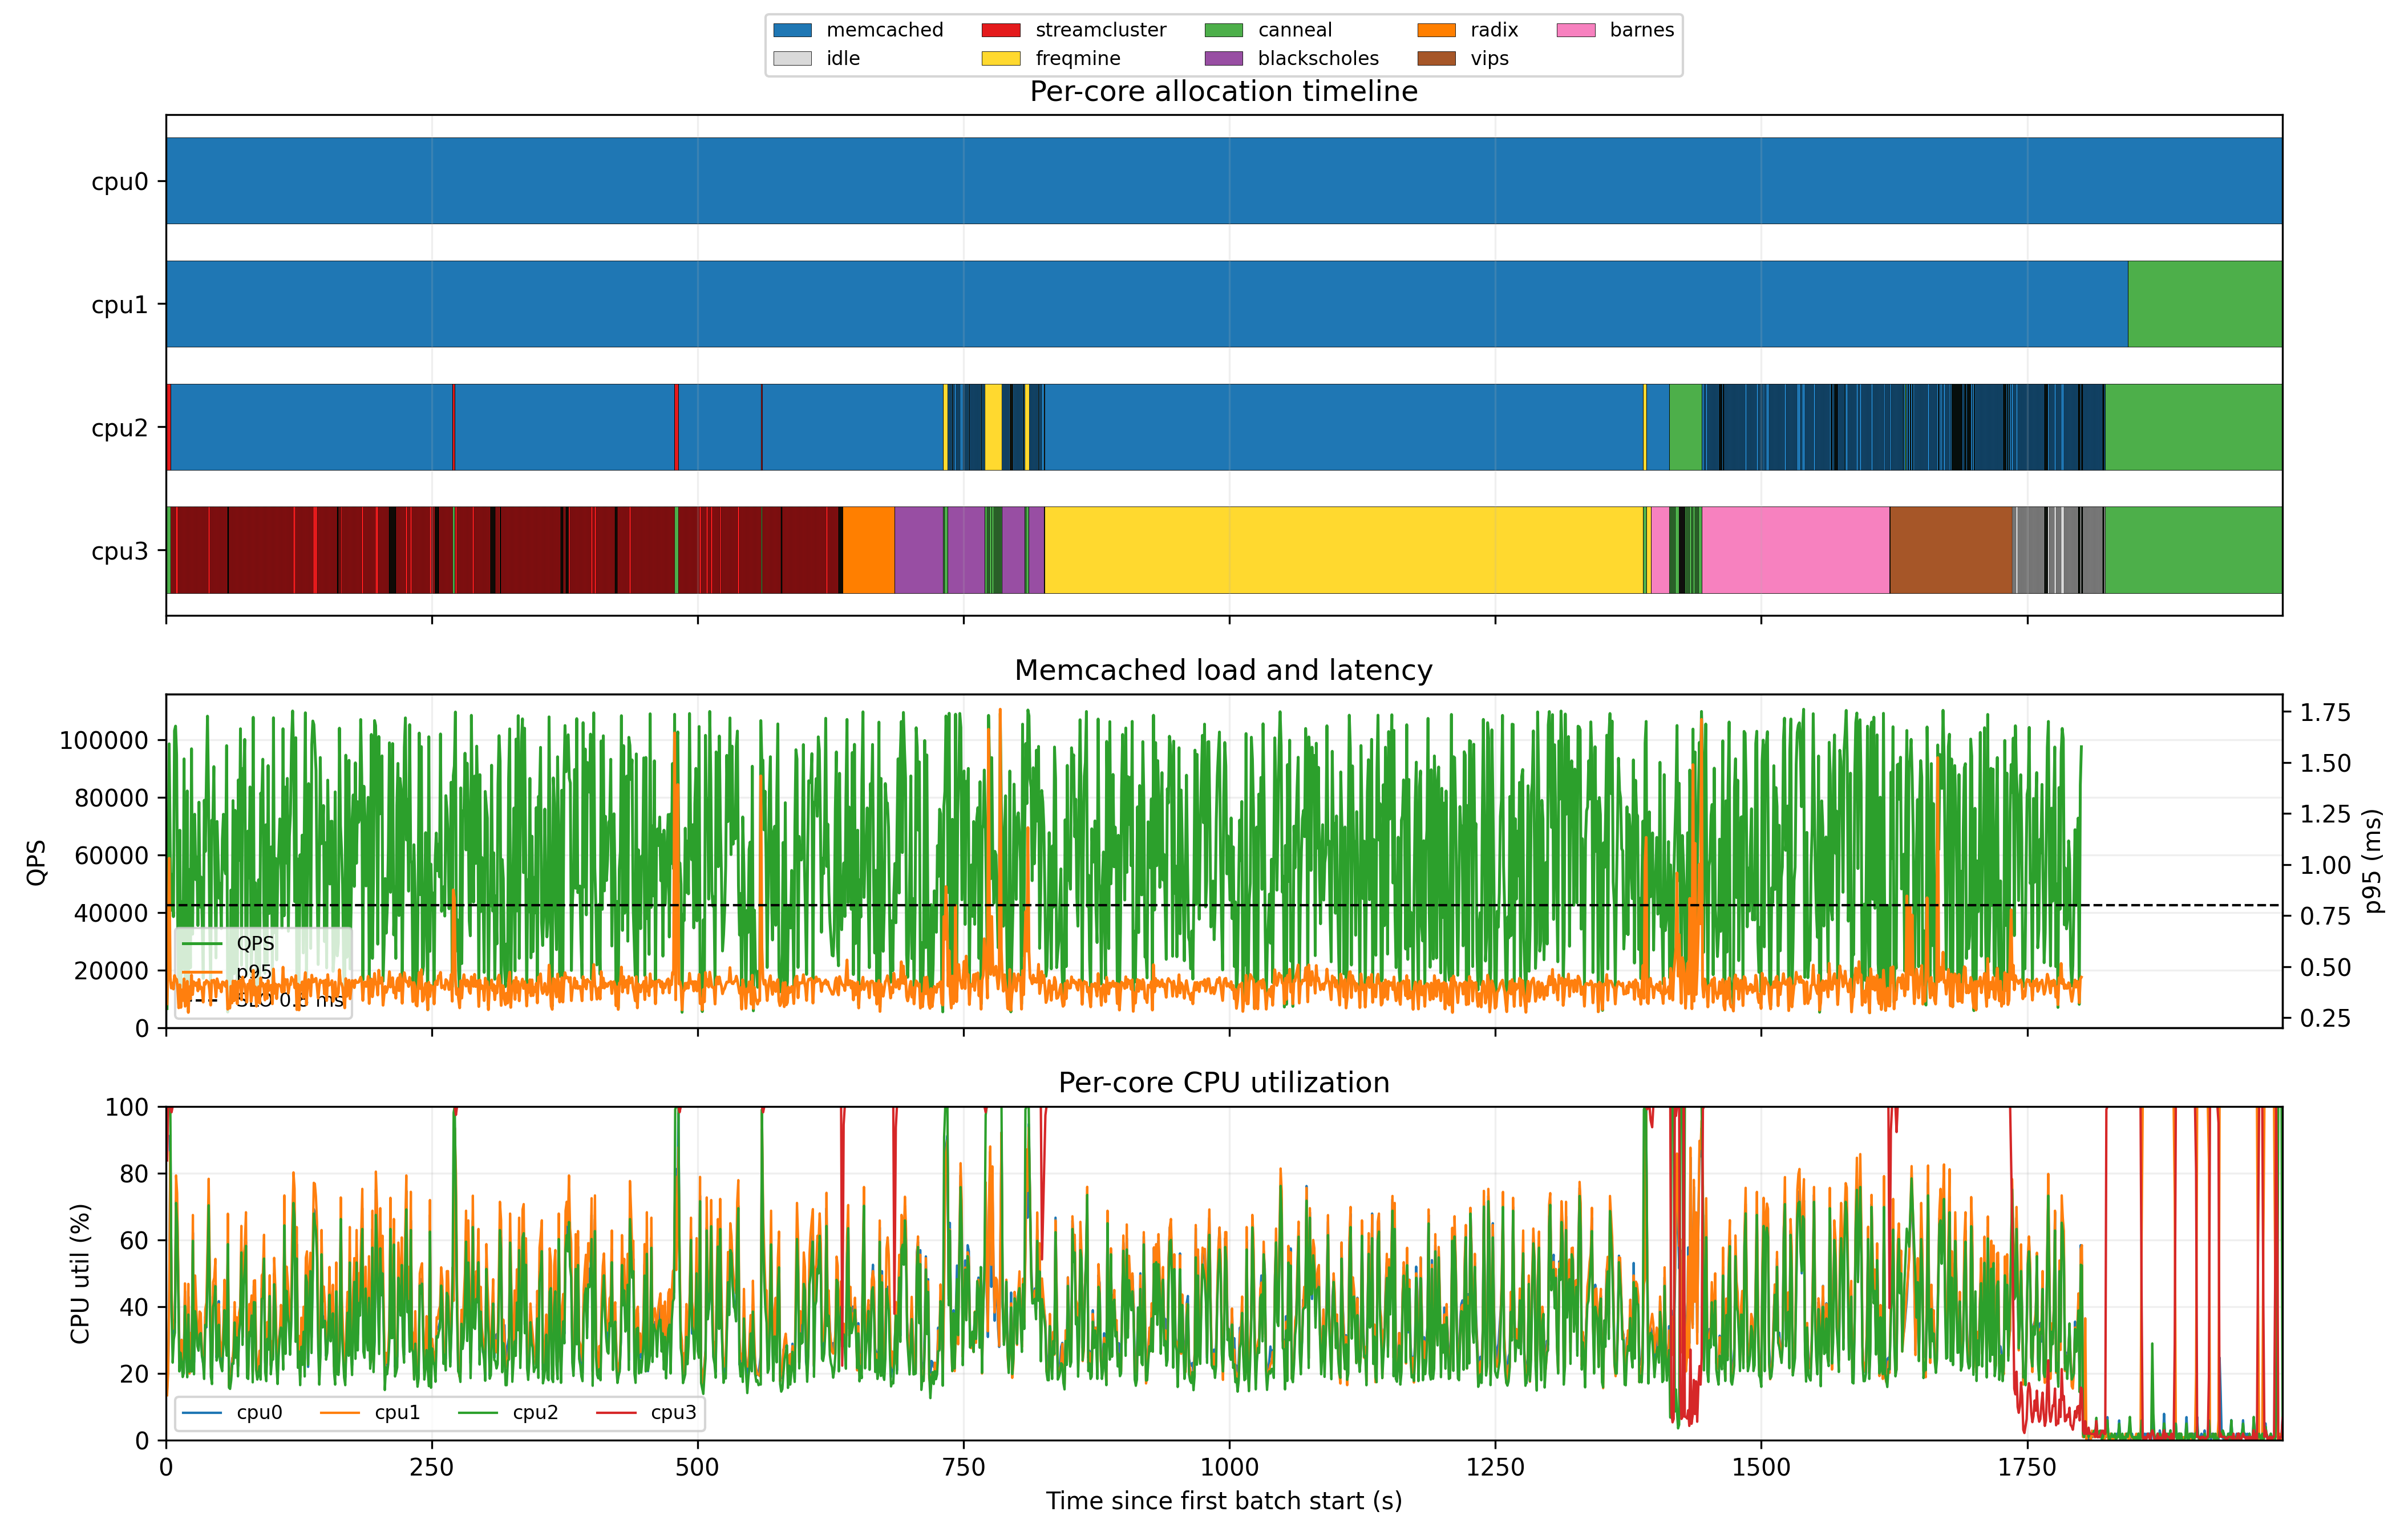
\includegraphics[width=0.75\linewidth]{figures/q4iv_run_1.png}
%     \caption{Q4.iv run 1.}
% \end{figure}

% \begin{figure}[H]
%     \centering
%     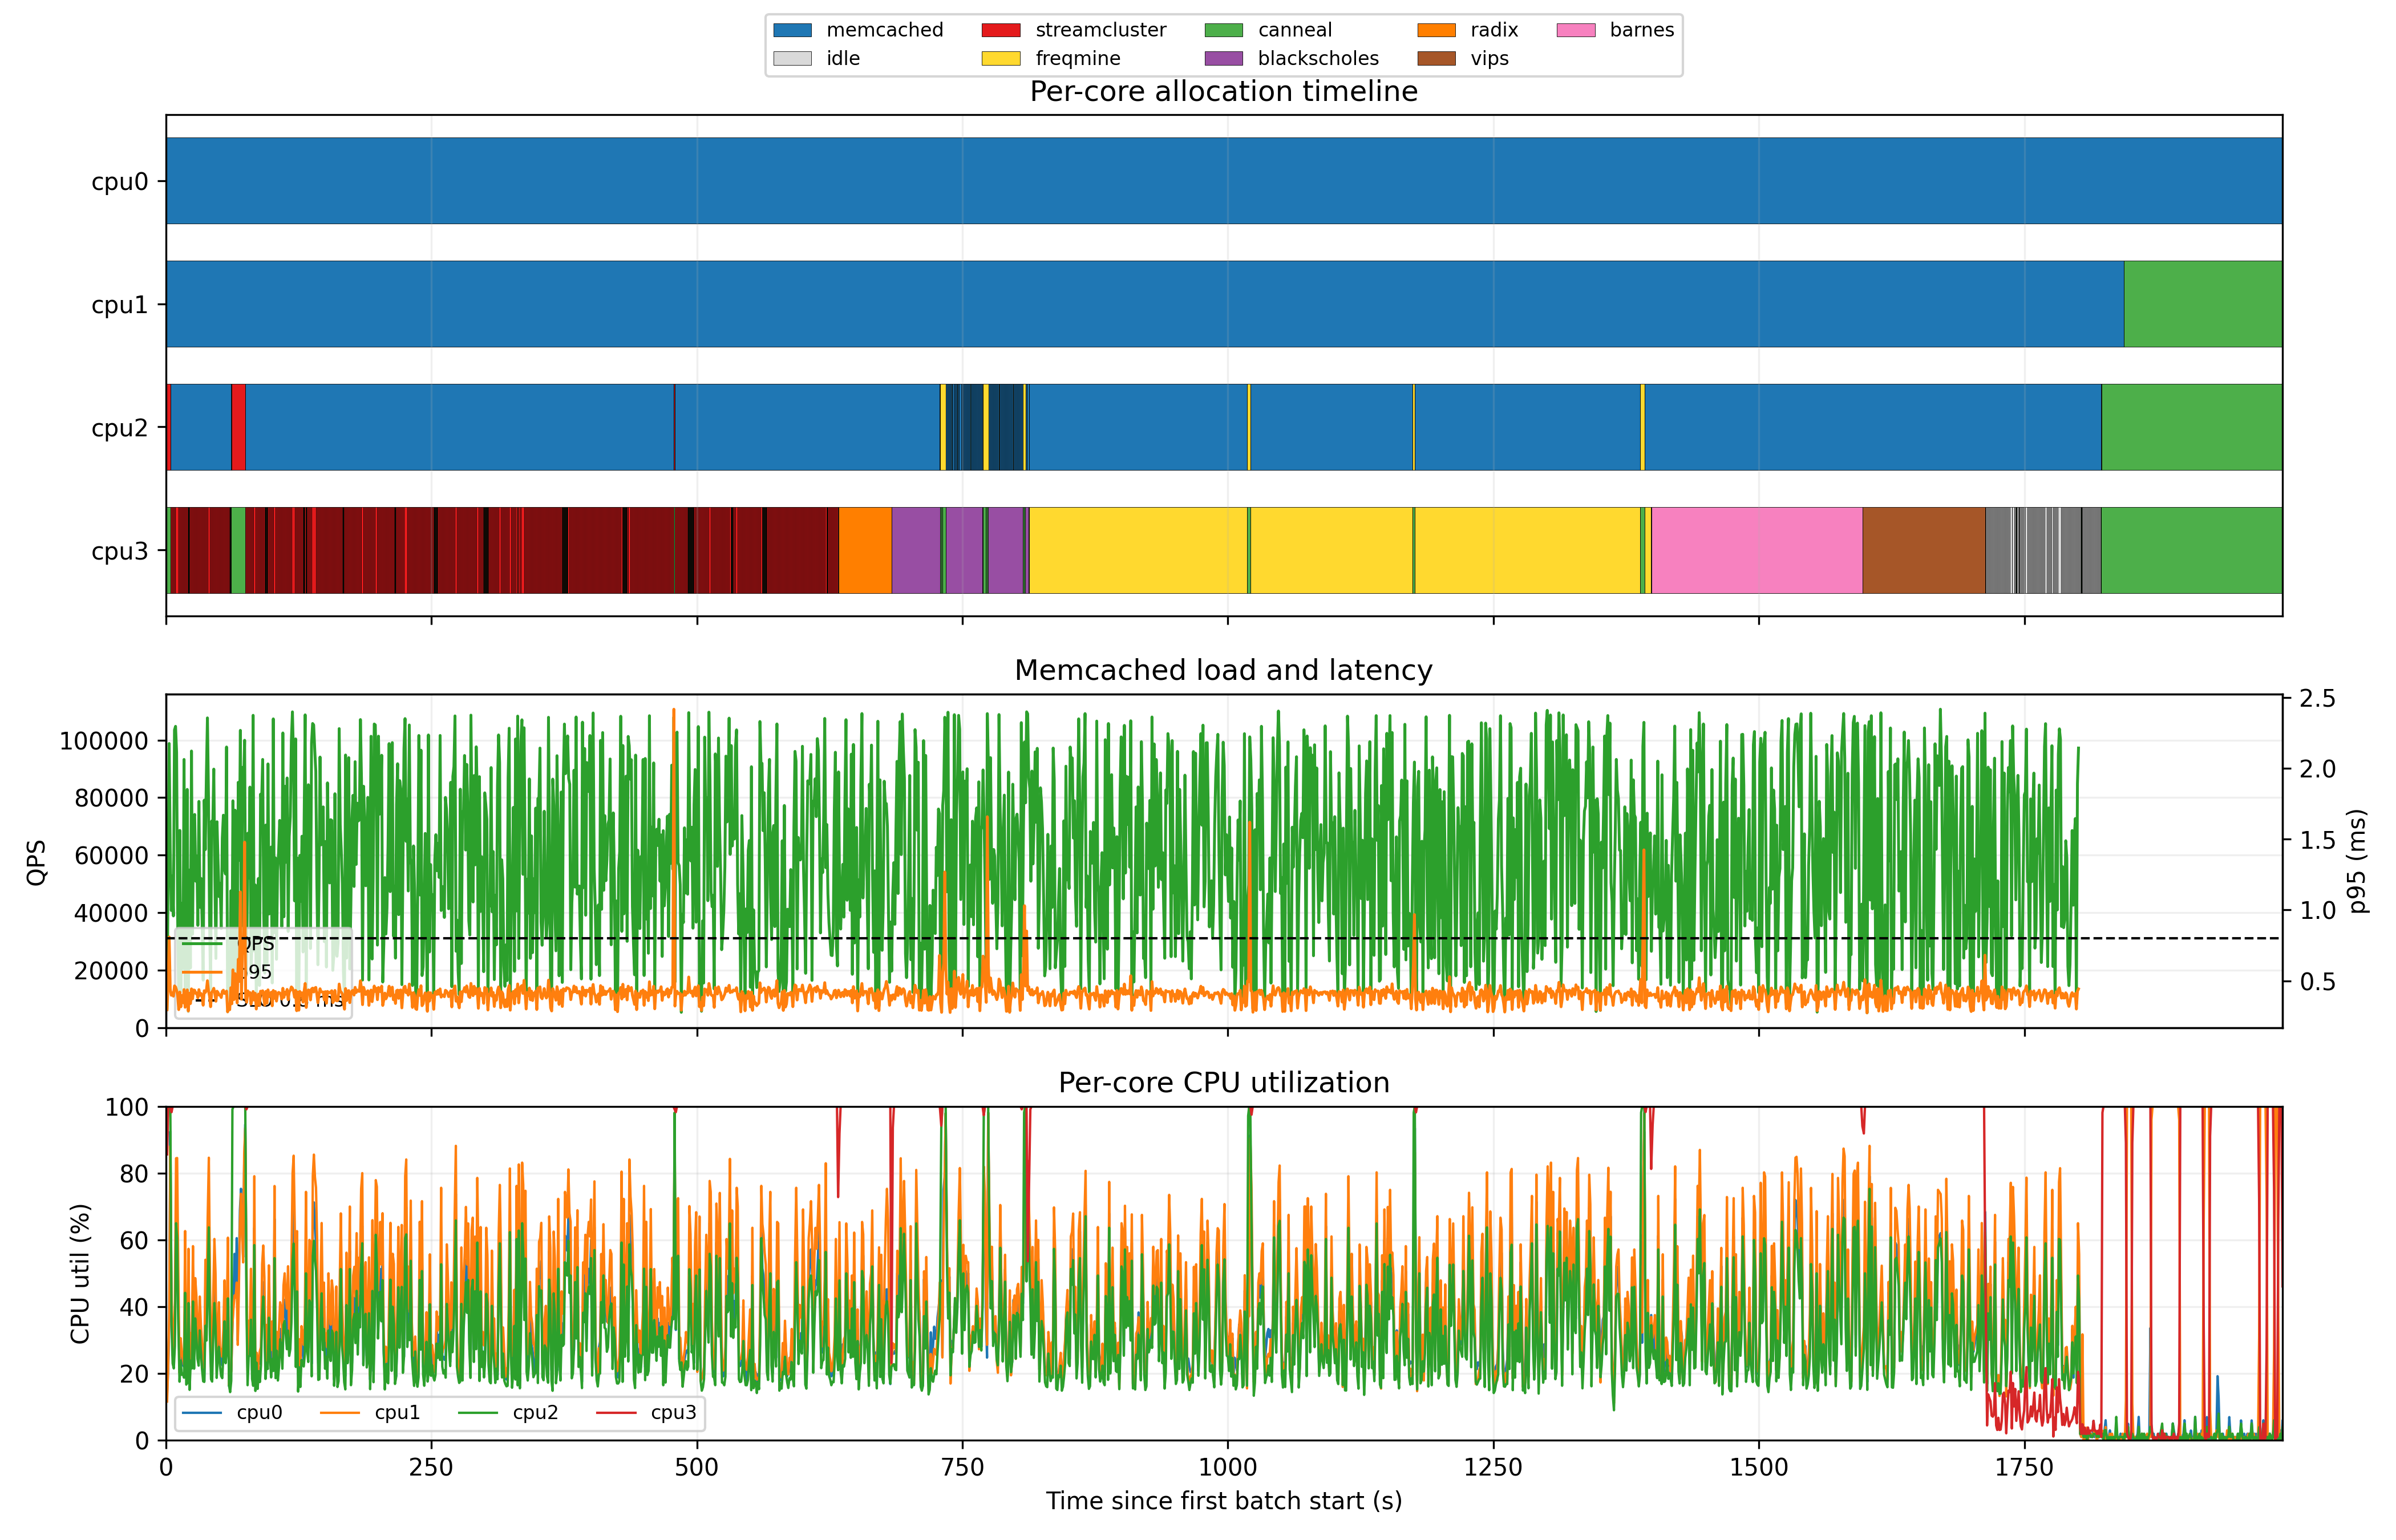
\includegraphics[width=0.75\linewidth]{figures/q4iv_run_2.png}
%     \caption{Q4.iv run 2.}
% \end{figure}

% \begin{figure}[H]
%     \centering
%     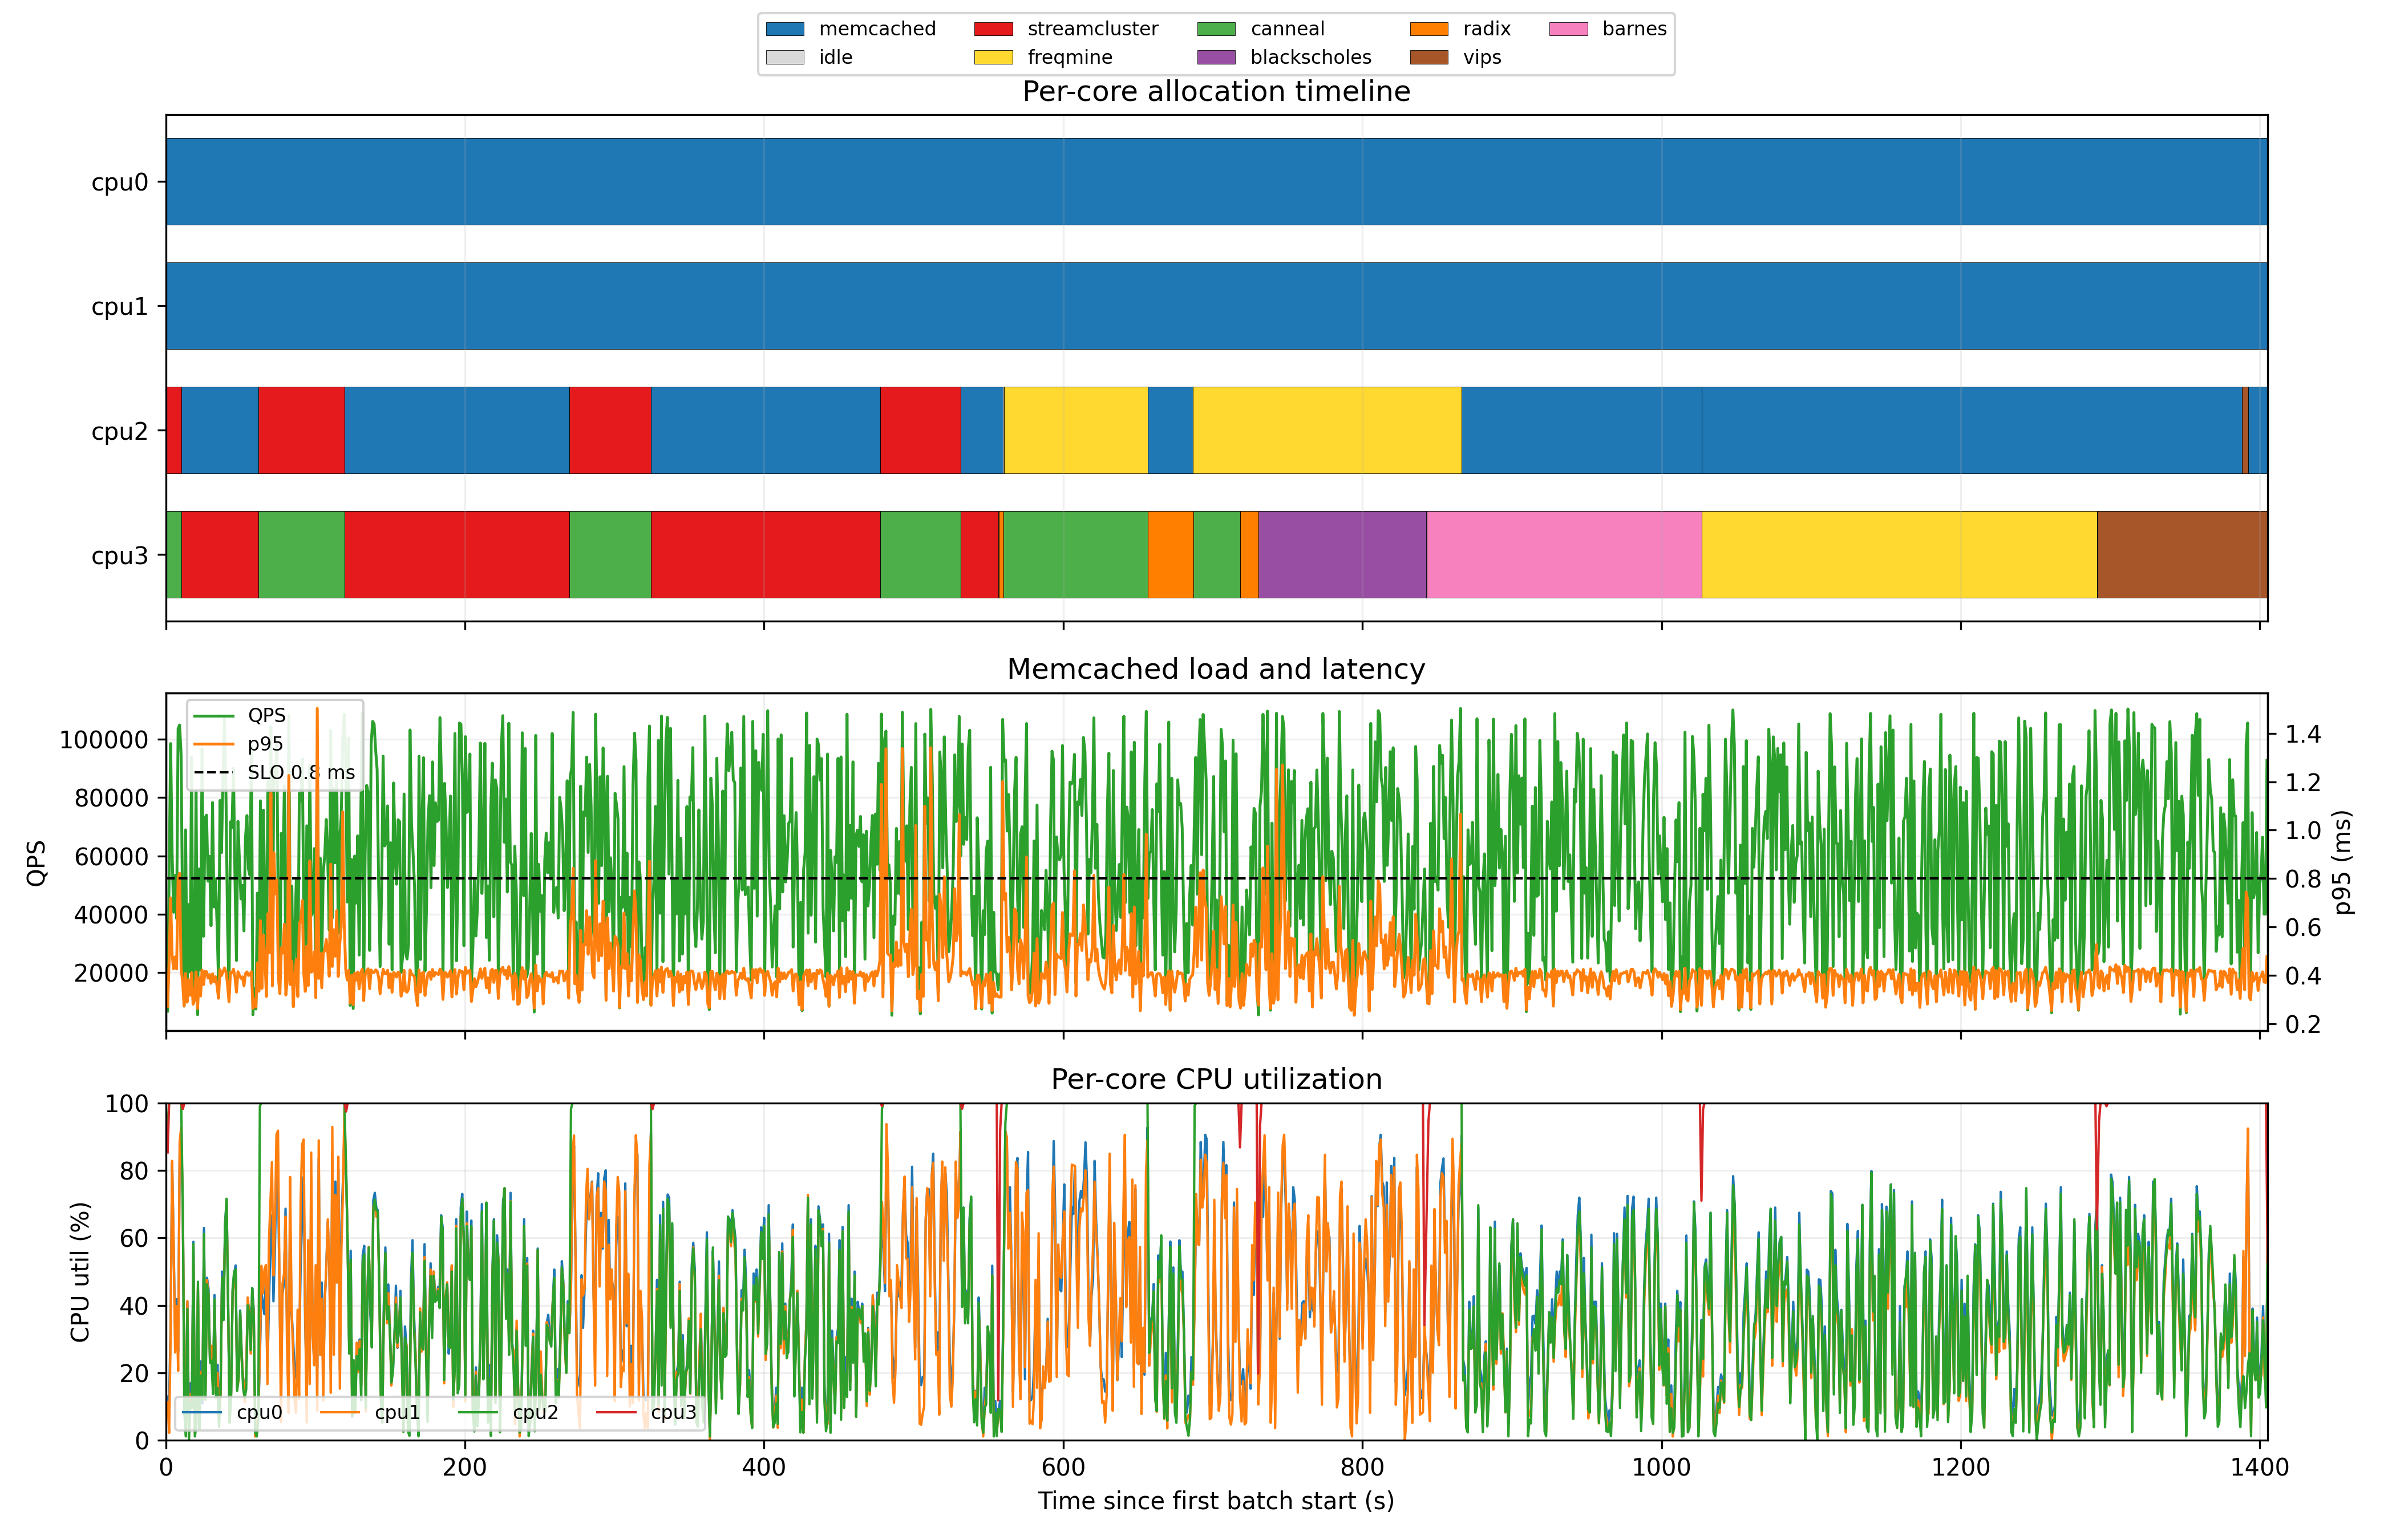
\includegraphics[width=0.75\linewidth]{figures/q4iv_run_3.png}
%     \caption{Q4.iv run 3.}
% \end{figure}

\end{enumerate}

\noindent
\textbf{\underline{Use of AI Tools}: Did you use any AI tools for this project? If so, disclose them here and explain what you used the tool(s) for and why. Note that the use of AI tools is NOT needed and NOT expected for the project.}

We used AI tools as programming assistance during the project. In particular, AI helped us draft and refine scripts to automate the experimental pipeline, including cluster setup commands, experiment orchestration, result parsing, plotting, and packaging. AI was also used to support parts of the controller implementation and debugging, such as improving robustness, and identifying issues in log parsing or time alignment. 
